\documentclass[12pt,oneside]{book}

% Long Table and decimal aligned columns
\usepackage{dcolumn}
\usepackage{longtable}

% Mathematics support
\usepackage{amsmath}
\usepackage{amsthm}
\usepackage{amssymb}


% Text Control
\usepackage{xspace}
\usepackage{textcase}

% Graphics
\usepackage{wasysym}
\usepackage{graphics}
\usepackage{graphicx}   % A package to allow insertion of
                        % external image files
\usepackage{csquotes}
\usepackage{float}
\pagestyle{headings}

% Note that the line below could be modified to suit a
% particular system since the "geometry" package behaves
% differently in Unix, Windows and Mac, especially for the
% top margins.
% Adjust the parameter "top" (measuring the height of the
% space allocated to a header) and "headsep" (measuring
% the distance from the bottom of the header to the
% first line of text.
\usepackage[top=1in,left=1.5in,bottom=1in,right=1in,headsep=0.5in]{geometry}

\usepackage{setspace}
%\onehalfspacing
\doublespacing

% Headers and footers for thesis
\usepackage{fancyhdr}

\markboth{}{}
\newcommand\startchapter[1]{\chapter{#1}\thispagestyle{myheadings}}
\newcommand\startappendix[1]{\chapter{#1}\thispagestyle{myheadings}}
\newcommand\startfirstchapter[1]{\chapter{#1}}

% Manual addition of section to Table of Contents
\newcommand\TOCadd[1]{\newpage\phantomsection\addcontentsline{toc}{chapter}{#1}}

% Float Customization
\renewcommand{\floatpagefraction}{0.01}

% Customization of Tables of Contents and List of Figures/Tables
\usepackage{tocloft}
\renewcommand\cfttabpresnum{Table\ }
\renewcommand\cfttabnumwidth{0.75in}
\renewcommand\cftfigpresnum{Figure\ }
\renewcommand\cftfignumwidth{0.80in}
\newcommand{\HRule}{\rule{\linewidth}{0.5mm}}

\graphicspath{{Figures/}}

\newenvironment{dedication}
{%\clearpage           % we want a new page          %% I commented this
	\thispagestyle{empty}% no header and footer
	\vspace*{\stretch{1}}% some space at the top
	\itshape             % the text is in italics
	\raggedleft          % flush to the right margin
}
{\par % end the paragraph
	\vspace{\stretch{3}} % space at bottom is three times that at the top
	\clearpage           % finish off the page
}

\def\citet#1{[\citeauthor{#1}, \citeyear{#1}]}
%\def\citet#1{\citep{#1}}

\begin{document}

% Front Matter
\input frontmatter/fm

\newpage

	\startfirstchapter{Introduction}
\label{chapter:introduction}

\input chapters/1/sec_intro
\input chapters/1/sec_review
%\pagebreak
\section{My Claims}
Something must be new in this work, no matter how small, since you are getting a graduate degree for it! Tell me about it clearly and succintly right now, just as you did in the abstract. Make an impact here. How about something like the following box:

I make \textit{four} claims which
my dissertation validates:
\\

\framebox{%
\parbox{5in}{
	My new algorithm to solve the problem of doing nothing include these important new features whose practical applicability can be proved both formally and empirically:
	\begin{enumerate}
	\item first feature;
	\item second feature;
	\item everything is much easier to understand, and therefore, easier to implement correctly.
	\end{enumerate}
}}
\\

\noindent Claim 1 and claim 2 are \textit{quantitative} - they will be proven by experiment.

\noindent Claim 3 is \textit{qualitative} - they will be demonstrated by argument.

\subsection{The Importance of My Claims}

Some very important positive consequences
arise from the validation of the above claims.
It is these consequences that comprise a significant
positive contribution to research in the field
of whatever the field is.
\\

\noindent Claim 1 implies that:
\begin{enumerate}
\item{Something profound which applies to:
	\begin{itemize}
	\item {something excellent;}
	\item {something important.}
	\end{itemize}}
\item{Something else just as profound.}
\end{enumerate}

\noindent Claim 2 implies that:
\begin{itemize}
\item{Repeat as above if necessary and useful.}
\end{itemize}

\noindent The consequence of claim 3 is that:
\begin{itemize}
\item{There must be something good coming out of all this work!}
\end{itemize}

\section{Agenda}

This section provides a map of the dissertation
to show the reader where and how it validates
the claims previously made. Here is where I am also presenting my own style of organization which may be totally different from what your supervisor thinks. However, trust me, this is a good solid beginning for a structure. Your supervisor may ask you to change it, but will still appreciate what you have! For each of the chapters below I also give a short summary of what the main focus should be and then I expand on it  a bit within the chapter itself.

\begin{description}
\item[\textbf{Chapter 1}] contains a statement of
the claims which will be proved by this dissertation followed by an overview of the structure of the document itself.
\item[\textbf{Chapter 2}] describes in details the open problem which is to be tackled together with its context, its impact and the overall motivation for the research overall.
\item[\textbf{Chapter 3}] gives the new research, its methodology, the algorithms involved, the new solution, the new work done. Formal proofs and arguments are made here. This is the first of the two contributions expected in a thesis for a graduate degree.
\item[\textbf{Chapter 4}] is where the experiments and the methodology for them is fully described. The first part includes all details of how the empirical side of the research has been conducted. Note that not every thesis has this empirical portion.
\item[\textbf{Chapter 5}] includes the evaluation of the data presented above and the comparisons with the work of others, to show how much better the new approach is. This is the second of the two contributions expected in a thesis for a graduate degree. Note that this part could be consolidated into the chapter above.
\item[\textbf{Chapter 6}] contains a restatement of the claims and results of the dissertation. It also enumerates avenues of future work for further development of the concept and its applications.
\end{description}

The list above is not complete. Chapter 3 actually includes a lot more, as I could not resist placing in it a few \LaTeX examples to help you along. This document is not a primer for \LaTeX, but there is no harm done in giving a little help.

	\startchapter{Related Works}
\label{chapter:problem}

\newlength{\savedunitlength}
\setlength{\unitlength}{2em}

Many variants of CAs have been proposed in a vast range of different applications such as single and multi-objective optimization, dynamic problems, social interactions simulation. Here, we are interested in studying socially motivated and multi-population variants as some modern approaches in solving optimization problems.
\subsection{Heterogeneous Multi-Population Cultural Algorithm}
[] proposed a new architecture for cultural algorithms. In this pproach, the whole population is divided into a set of independent sub-populations which work in parallel without direct communication. They referred to the works of [] [] [] []. As their motivation they stated that most of proposed variants of evolutionary algorithms suffers from immature convergence. This occurs because these algorithms can not hold the diversity at a reasonable level. Based on existing research works, they hypothesized that multi-population streategies would be a better choice as they have the potential to perfrom an efficient search on complex landscapes. In their approach, the optimization parameters are divided among some heterogenous sub-populations. the sub-populations are called heterogenous because each sub-population is responsible for optimizing a different subset of parameters. Each sub-population represents a partial solution instead of a complete solution. To evaluate a partial solution, it gets completed by its complement parameter values from the belief space. The complete solution is evaluated based on a numerical optimization function. Also, to make the convergence process faster a simple local search strategy is incorporated into the proppsed algorithm. The general architecture of their algorithm is presented in figure ???\newline
In the experiments, they considered the whole population size to be 1000 individuals. It is divided into 30 sub-populations. So, the size of each sub-popualtion is 33. The algorithm runs for the maximum of 10000 generations and the local search strategy runs only for 10 iterations. They evaluated HMP-CA on a set of 8 complex optimization functions. It is able to find the minimum value for 7 functions out of 8. However, when the local search strategy is applied to the expriments, the proposed method outperforms all of the functions and it finds the optimum value very quickly. Ultimately, they claimed that their porpsed approach is efficient in both time and space complexity.

\subsection{The Social Fabric Approach as an Approach to Knowledge Integration in Cultural Algorithms}	
[] begins with a brief introduction to socially motivated methods to problem solving. It compares qualities of Ant Colony Optimization (ACO), Particle Swarm Optimization (PSO), and Cultural Algorithms (CA) regarding the scale in which the interactions between agents occur. Figure (()) compares PSO, ACO, and CA in terms of the time and space continuum over which the social interactions occur. Individuals in ACO and PSO tend to interact in a reatively limited temporal and spatial scales. It is obvious because the agents in both ant and paricle swarm algorithms exchange information with only other agents in their local neighborhood. On the other hand, cultural algorithms let the individuals interact together using various types of symbolic information emerged from complex cultural systems. In cultural algorithms the interactions among individuals occur indirectly through a shared belief space. So, cultural algorithms allow individuals interact in a global scale.\newline
Then, they asked the essential question of what social structures might emerege alongisde the search process?. To answer such questions, they introduced a new influence function which utilizes the social fabric phenomena. The old influence function assumes no interactions between agents and works based on the simple roulete wheel method. On the other hand, in the new influence function, the individuals are connected through a social network (fabric). Multiple layers of such networks could be employed in a population. The interplay of these network connection forms a social fabric. At each iteration, an individual could specify its controller knowledge source. In this approach, the contoller knowledge source is chosen based on the majority of knowledge sources in the neighborhood of an individual. The neighborhood size of an individual is specified by the topology of the fabric. Inspired by Particle Swarm Optimization literature, different topologies could be taken into consideration to model the relationships among individuals. In their work, they only considered Ring and Square topologies. They stated that, the topology of the social fabric determines the extent to which the influence of knowledge sources could be spread thorugh the network.\newline
To evaluate the social fabric approach, they implemented it in Repast frameork. Repast is a simuation tool for multi-agent systems. They created a cultual algorithms toolkit (CAT) to view the capabilities of cultural algorithms in solving various problems. They chose Cone World problem to evaluate and compare their approach with the standard cultural algorithm. The reason that they chose this problem is that by changing its parameters during the evolution process, it can show a dynamic behavior. So, Cone World problem provides an efficient way to test flexibility of search algorithms. They set the parameters of CAT as: 100 individuals, 100 cones and 1000 generations. They used ring and square topologies to from he social fabric. They stated that square topology works better than ring as it finds the solution after 250 iterations. While, the ring topology finds the best solution 450 iterations.
\subsection{Robust Evolution Optimization at the Edge of Chaos: Commercialization of Culture Algorithms}
The authors of [] aimed at commercializing Cultural Algorithm Toolkit (CAT) thourgh developing a robust variant of it. By robustness, they mean to develop a cultural algorithm which is capable of being applied across a vast range of complex problems. At first, they referred to [Peng model] as an standard model cultural algorithms which assumes no connection between individuals. Then, they referred to [Ali], which introduced the concept of social fabric to allow individuals interact together. The authors extended the work of Ali 

\newline------------------------------\newline

\newline

\newline

Here is where you tell me what is the problem you have been working on for the past few months (or years). I want all the details and you should not be timid about being too tutorial, except that you do not want to cross the line towards writing a textbook. However consider carefully that \textit{communication} implies conveying ideas to other people, while \textit{effective communication} occurs when your message is clearly understood. Remember that your audience must understand your message before they can agree with you.

Ask yourself:
\textit{who is your audience?} You might think of your supervisor who knows everything and you want to impress with your knowledge. I think instead of the graduate students who will be reading this thesis which is, after all, a property of the university. It is published as a university technical report so that others may learn by reading it. Then teach them! Be a bit tutorial. Even the expert external examiner will be impressed by your clarity of exposition if he or she does not need to read paragraphs twice in order to understand - something which people with PhDs and big egos find particularly irritating.

On the other hand, do not go too far and give trivial definitions from concepts learned in a 3rd year undergraduate courses, else you might find yourself in trouble when having to remember the details during an oral examination.

My approach is to put everything necessary to make clarity for
the problem the main goal of this chapter, assuming an intelligent and well prepared reader who already has a Bachelor degree in an appropriate subject.

Once I understand the problem clearly and its nuances (it may not be what I expected after all), I also need to know why the problem is important, what its impact is and what its application, if any. Here you are free to elaborate and write as much as you think is necessary to avoid the examination doubt that you have a brilliant new solution to a trivial and unimportant issue.

I suggest reading various books on how to do research and set up problems. The best for me was "The Craft of Research" by Wayne Booth \cite{booth1}, which can be found in the main library at Q180.55 M4B66. From there I have transferred to my writing a fairly simple structure for talking about the topic of the research, with the question to be asked and its motivation and significance. It goes as follows:
\begin{enumerate}
\item {\textit{I am trying to learn about (working on, studying...)}}
\item {\textit{because I want to find out....}}
\item {\textit{in order to understand...}}
\end{enumerate}

Another way of looking at this is to ask the
\textit{what}, \textit{why} and \textit{where}, starting from a \textit{setting} of the problem with a first point A, stating what the \textit{goal} is at point B and having an \textit{action link} between the two which will encompass your new solution. As surprising as this may be to some of you, I found reading a book from Microsoft very useful: "Beyond Bullet Points: Using Microsoft Office PowerPoint 2007 to Create Presentations That Inform" \cite {atkin}. The goal of the book is to improve presentations with Power Point, but there is a lot that can be transferred towards \textit{effective communication} for a thesis.

In summary, my view of the second chapter on
\textit{"The Problem to be solved"} is as follows:
\begin{enumerate}
\item {\textit{Not} all the background and definitions (boring!) - use instead just-in-time explanations as needed in every context as it comes up;}
\item {Motivation in depth;}
\item {Tutorial high level explanation, where it is important to choose the right pitch: who is the audience? who are you teaching here?}
\item {Make it exciting, make it current, make it important - why do I want to keep reading?}
\item {Should you list here the solutions from other researchers? I think not, list instead the different facets of the problems that other researchers have attacked.}
\item {A taxonomy can be extremely useful to place your problem and its particular special features within the perfect context of the overall area, as you need to make sure that the reader understands perfectly what you are trying to solve.}
\end{enumerate}


\setlength{\unitlength}{\savedunitlength}

	\startchapter{The New Approach and Solution}
\label{chapter:newsol}

This is where you go all out and tell us all about your new discovery and research related to the problem in the previous chapter. No arrogant sweeping statements which cannot be fully justified, but no false modesty either. You must impress your reader that you have accomplished something.

Simply summarized, this chapter should be comprised of at least two main sections, each with appropriate subsections. The first section should describe:
\begin{itemize}
\item {what the new approach is;}
\item {what is really totally new;}
\item {what is incrementally new;}
\item {what you built upon.}
\end{itemize}

The second part should describe fully how the new approach works, both with the overall theoretical exposition (e.g. an algorithm) and with as many examples as necessary for clarity. Remember that if the reader does not understand fully, you will get a lot of questions and doubts. Good examples, good figures, good diagrams with super clear tutorial explanations can be a joy to read and make even a small contribution appear to be more impressive. Are you afraid that if you are too tutorial your work will not seem as deep and difficult? Only shallow people will make such a superficial evaluation, have trust instead in the wisdom of your supervisory committee.

Use at least one good example throughout, and even better if this is one of the examples you used in Chapter 2 to describe the original problem.

By the way, this would be the first chapter I would write. This is what I know best right now, as I just finished working on it. It is clear to me and on the tip of my fingers. Start with your strengths! The second chapter I would write is the next one about the experiments, followed closely by chapter 2 describing the problem. It may not seem intuitive to you, but it works and it is the most productive way I ever found to finish a document.


\input chapters/3/sec_latexhelp

	\startchapter{Proposed Approaches: Improving Robustness in Social Fabric}
\label{chapter:Exp}
Inspired by natural systems, many evolutionary algorithms have been proposed to solve various optimization problems. These algorithms are expected to exhibit a consistent problem-solving behavior against different optimization landscapes. Unfortunately, as stated by No Free Lunch (NFL) theorem \cite{wolpert1997no}, there is no algorithm better than others over all cost functions. It means, there is no guarantee for an algorithm to work well for all functions if it shows promising results for a particular category of them. Therefore, robustness has been one of the most desired features which motivates researchers to invent new methods which are less dependent on the kind of a problem than others. Here, robustness means we need to develop search strategies which are capable of adapting themselves across different landscapes which might vary regarding aspects such as multimodality and the number of local optima. 
\newline
In this section, we are going to improve the robustness of CAs in both population space and belief space components. In the population space, a new neighborhood restructuring strategy will be proposed which aims at microscopic inspections for stagnation regarding individuals' local experience. Then, in the belief space, a new model of Normative KS will be proposed, which defines the normative ranges based on Confidence Interval inspired from Inferential Statistics. It stops the normative KS to be affected by sudden fluctuations in the input data.

\section{Self-organization}
A self-organized system is a group of agents with specific behavioral patterns which could not be predicted from the simple behaviors of the  individuals who make up the system. Kennedy and Eberhart [] described self-organization as follows: 
\begin{displayquote}
	"Self-organization The ability of some systems to generate their form without external pressures, either wholly or in part. It can be viewed as a system’s constant attempts to organize itself into ever more complex structures, even in the face of the constant forces of dissolution described by the second law of thermodynamics."
\end{displayquote}
Some of the primary attributes of self-organizing systems are listed below:
\begin{enumerate}
	\item Self-organizing systems usually exhibit the behaviors that appear to be spontaneous order.
	\item Self-organization can be considered as a system’s constant attempts to organize itself into a variety of complex structures, even in the face of the forces of deviation (Robustness).
	\item The overall status of a self-organizing system is an emergent property of all the ingredients of the system.
	\item Interconnected components of the system become organized in a meaningful way based on local interactions of the components.
	\item Complex systems have the potential to self-organize themselves.
	\item The self-organization process works close to the “edge of chaos.”
\end{enumerate}
In the section, we will propose a new approach to improve the robustness of cultural algorithms regarding self-organization.
\section{Irregular Neighborhood Restructuring}
As proposed by \cite{ali2016leveraged}, when the agents of a tribe get stuck in a local optimum, then they choose a topology with fewer connections such as ring topology to motivate exploration. When the agents lack information, the topology is changed to a denser topology like Mesh, and ultimately Global. Whenever a tribe does not make progress for $M_{thresh}$ iterations, then the algorithm decides on upgrading/downgrading the current topology to other topologies. Downgrading happens by moving in the direction of gbest$\rightarrow$tree$\rightarrow$mesh$\rightarrow$lbest and Upgrading occurs in the direction of lbest$\rightarrow$mesh$\rightarrow$tree $\rightarrow$gbest. In our proposed approach, the restructuring process occurs at a microscopic level. There is no daemon process for inspecting stagnation. Every agent checks its performance for stagnation. If it gets stuck in a local optimum, it decides to upgrade/downgrade its neighborhood. The proposed strategy is described in the algorithm \ref{ref:RNR}. If the particle is the best in its neighborhood, it starts to decrease the number of connections to motivate exploration. However, if it is not the best, it needs to increase the neighborhood size to facilitate exploitation. Here, the topology is dynamic and irregular and the neighborhood size is different for each agent. So, it could be considered as a heterogeneous variant of CAs \cite{de2009heterogeneous}. The ultimate topology of the fabric is formed through local interactions of the agents. In this way, it improves the robustness of CAs regarding self-organization concept \cite{kennedy2001swarm}.

\section{Confidence based Normative Knowledge Source}
The current version of Normative KS is quite vulnerable to temporary fluctuations in the pattern of input data. The size of Normative ranges is subject to change dramatically with any temporal fluctuations. In this section, we are going to replace the ranges in the standard Normative KS with Confidence Interval from Inferential Statistics. Confidence-based changes are more robust against instantaneous changes in the input pattern. The update process of standard normative ranges is as follows:
\begin{equation}
lb_{j}(t+1) = \begin{cases} x_{i,j}(t), & x_{i,j}(t)\leq lb_{j}(t)\:or\:f(X_{i})<PL_{j}(t)  \\ lb_{j}, & \mbox{otherwise} \end{cases}
\end{equation}

\begin{equation}
ub_{j}(t+1) = \begin{cases} x_{i,j}(t), & x_{i,j}(t)\ge ub_{j}(t)\:or\:f(X_{i})<PU_{j}(t)  \\ ub_{j}, & \mbox{otherwise} \end{cases} 
\end{equation}%\newline
The following is the definition of normative ranges based on Confidence Interval concept \cite{proakis1985probability}.
%\begin{equation}
%	(\bar{x}_{j}-q\cdot\dfrac{\sigma_{j}}{\sqrt{n}} , \bar{x}_{j}+q\cdot\dfrac{\sigma_{j}}{\sqrt{n}}) 
%\end{equation}
\begin{equation}
lb_{j}=\bar{x}_{j}-q\cdot\dfrac{\sigma_{j}}{\sqrt{n}}
\end{equation}
\begin{equation}
ub_{j}=\bar{x}_{j}+q\cdot\dfrac{\sigma_{j}}{\sqrt{n}}
\end{equation}
where 
$\bar{x}_{j}$ is the mean of $j$th dimension, $\sigma_{j}$ is the standard deviation of $j$th dimension and $q$ is the confidence coefficient \newline
\newline ----------------------- \newline





%Assuming you have some experimental results to support your claims this is where all the data is reported. There are a few issues you should consider before dumping a lot of stuff here, or it will lose its effectiveness.
%
%First of all you must describe precisely the experimental setup and the benchmarks you used. In any scientific discipline an experimental result is only good if it is reproducible. To be reproducible then somebody else must have sufficient details of the setup to be able to obtain the same data. Thus the first section in this chapter is a super precise history of the decisions made towards experimentation, including mentions of the paths which became infeasible. The setup must be valid and thus your description of it must prove that it is indeed sound. At times, terrifying times, when writing this section, both supervisor and student realize belatedly that something is missing and more work needs to be done!
%
%The second portion of this chapter is dedicated the the actual results. At least two issues arise here:
%\begin{enumerate}
%\item {Should all the data be reported here or should some be placed in the Appendix?}
%\item {Should this be an exposition of the raw facts and data or should it include its analysis and evaluation?}
%\end{enumerate}
%
%There are no definite answers here, but I follow a few rules.
%
%\textit{Should all the data be reported here or should some be placed in the Appendix?}
%    \begin{itemize}
%    \item{If there is a large number of tables of data, it might be better to present here only a handful of the most significant ("best") results, leaving all the rest of the data in the Appendix with proper linkages, as it would make the chapter so much more easily readable (not to mention limiting the struggle with a word processor for the proper placement of tables and text).}
%    \item{Use an example throughout, call it a "case study" to make it sound better, so that all the data and results are somehow linked in their logic, and even better if this is one of the examples you used in Chapter 2 to describe the original problem.}
%    \item{Highlight in some manner the important new data, for example the column of your execution speed where all the numbers are much smaller. Make the results highly easy to read!}
%    \item{It is normally expected that data should be presented only in one form and not duplicated, that is, you are not supposed to include both a table of raw numbers and also its graphical representation from some wonderful Excel wizard. I tend to disagree. I would not wish to see every results repeated in this manner, but some crucial ones need to be seen in different manners, even with the same information content, in order to show their impact. One good trick is to place the more boring tables in the Appendix and use wonderful graphs in this chapter.}
%    \item{This is the one chapter where I would splurge and use colour printing where necessary, as it makes an \textit{enourmous} difference.}
%    \end{itemize}
%
%\textit{Should this be an exposition of the raw facts and data or should it include its analysis and evaluation?}
%     \begin{itemize}
%    \item{Is the evaluation of the data really obvious? For example you have 10 tables to show that your chemical process is faster in development and gives purer material - you may simply need to highlight one column in each table and state the obvious.}
%    \item{Most results are not that obvious even if they appear so. Moreover this is where you are comparing your \textit{new} results to data from other people. I usually describe other people's work at this point and make comparisons. That is why I prefer to talk about the analysis and evaluation of the results in a separate chapter.}
%    \item{There is absolutely no clear structure here which is best.}
%    \end{itemize}
%
	\startchapter{Experimental Setup}
\label{chapter:eval1}
In this chapter, we explain the experimental setup, how to set the parameters and the optimization functions as the benchmark to evaluate the efficiency of our proposed approaches. 
\section{Description}
In this section, we describe IEEE-CEC2015 as the function set which we have chosen for our benchmark optimization purpose. IEEE-CEC2015 is a set of 15 functions with different properties such as multi-modality, copious local optima, and non-separability. All test functions are minimization problems defined as follows:
\begin{equation}
Y=f(x_{1}, x_{2}, x_{3}, \cdots, x_{D})
\end{equation}
where $D$ is the number of dimensions.\newline
Before evaluation, all the vectors are shifted and rotated as described in [].$\mathbf{o}_{i}=[o_{i}{1}, o_{i}{2},\cdots, o_{i}{D}]$ is the shifted global optimum, which is randomly distributed in [-80,80] D For convenience, the same search ranges are defined for all test functions as $[-100, 100]^{D}$
\section{Benchmark Functions}
In this section, we describe the IEEE-CEC2015 functions and their properties as a well-known benchmark adopted by many researchers to evaluate innovative ideas in solving complex optimization problems. 
\subsection{Unimodal Functions}
\subsubsection{Rotated Bent Cigar Function}
\begin{equation}
	f_{1}(x)=x_{1}^{2}+10^{6}\sum_{i=2}^{D}x_{i}^2
\end{equation}
\begin{equation}
	F_{1}(x)=f_{1}(M(x-o_{1}))+F_{1}^{*}
\end{equation}
Properties:
\begin{enumerate}
	\item Unimodal
	\item Non-separable
	\item Smooth but narrow ridge
\end{enumerate}

\subsubsection{Rotated Discus Function}
\begin{equation}
	f_{2}(x)=10^{6}x_{1}^{2}+\sum_{i=2}^{D}x_{i}^2
\end{equation}
\begin{equation}
	F_{2}(x)=f_{2}(M(x-o_{2}))+F_{2}^{*}
\end{equation}
Properties:
\begin{enumerate}
\item Unimodal
\item Non-separable
\item With one sensitive direction	
\end{enumerate}

\subsection{Simple Multimodal Functions}
\subsubsection{Shifted and Rotated Weierstrass Function}
\begin{equation}
	f_{3}(x)=\sum_{i=1}^{D}(\sum_{k=0}^{kmax}[a^{k}\cos(2\pi b^{k}(x_{i}+0.5))])-D\sum_{k=0}^{kmax}[a^{k}\cos(2\pi b^{k}\cdot 0.5)]
\end{equation}
where a=0.5, b=3, and kmax=20.
\begin{equation}
	F_{3}(x)=f_{3}(M(\frac{0.5(x-o_{3})}{100}))+F_{3}^{*}
\end{equation}
Properties:
\begin{enumerate}
\item Multi-modal
\item Non-separable
\item Continuous but differentiable only on a set of points	
\end{enumerate}
\subsubsection{Shifted and Rotated Schwefel's Function}
\begin{equation}
	f_{4}(x)=418.9829 \times D - \sum_{i=1}^{D}g(z_{i}), z_{i}=x_{i}+4.209687462275036e+002
\end{equation}
\begin{equation}
	F_{4}(x)=f_{4}(M(\frac{1000(x-o_{4})}{100}))+F_{4}^{*}
\end{equation}
Properties:
\begin{enumerate}
\item Multi-modal
\item Non-separable
\item Local optima's number is huge and second better local optimum is far from the global optimum.
\end{enumerate}

\subsubsection{Shifted and Rotated Katsuura Function}
\begin{equation}
	f_{5}(x)=\frac{10}{D_{2}}\prod_{i=1}^{D}(1+i\sum_{j=1}^{32}\frac{|2^{j}x_{i}-rand(2^{j}x_{i})|}{2^{j}})^{\frac{10}{D^{1.2}}}-\frac{10}{D^{2}}
\end{equation}
\begin{equation}
	F_{5}(x)=f_{5}(M(\frac{5(x-o_{5})}{100}))+F_{5}^{*}
\end{equation}
Properties:
\begin{enumerate}
	\item Multi-modal
	\item Non-separable
	\item Continuous everywhere yet differentiable nowhere
\end{enumerate}

\subsubsection{Shifted and Rotated HappyCat Function}
\begin{equation}
	f_{6}=|\sum_{i=1}^{D}x_{i}^2-D|^{0.25}+\frac{0.5\sum_{i=1}^{D}x_{i}^{2}+\sum_{i=1}^{D}x_{i}}{D+0.5}
\end{equation}
\begin{equation}
	F_{6}(x)=f_{6}(M(\frac{5(x-o_{6})}{100}))+F_{6}^{*}
\end{equation}
Properties:
\begin{enumerate}
	\item Multi-modal
	\item Non-separable	
\end{enumerate}

\subsubsection{Shifted and Rotated HGBat Function}
\begin{equation}
	f_{7}=|(\sum_{i=1}^{D}x_{i}^2)^{2}-(\sum_{i=1}^{D}x_{i})^{2}|^{0.25}+\frac{0.5\sum_{i=1}^{D}x_{i}^{2}+\sum_{i=1}^{D}x_{i}}{D+0.5}
\end{equation}
\begin{equation}
	F_{7}(x)=f_{7}(M(\frac{5(x-o_{7})}{100}))+F_{7}^{*}
\end{equation}
Properties:
\begin{enumerate}
	\item Multi-modal
	\item Non-separable	
\end{enumerate}

\subsubsection{Shifted and Rotated Expanded Griewank's plus Rosenbrock's Function}
\begin{equation}
	f_{8}(x)=f_{11}(f_{10}(x_{x_{1}, x_{2}}))+f_{11}(f_{10}(x_{x_{2}, x_{3}}))+\cdots+f_{11}(f_{10}(x_{x_{D-1}, x_{D}}))+f_{11}(f_{10}(x_{x_{D}, x_{1}}))
\end{equation}
\begin{equation}
	F_{8}(x)=f_{8}(M(\frac{5(x-o_{8})}{100})+1)+F_{8}^{*}
\end{equation}
Properties:
\begin{enumerate}
	\item Multi-modal
	\item Non-separable	
\end{enumerate}

\subsubsection{Shifted and Rotated Expanded Scaffer's F6 Function}
\begin{equation}
	g(x,y)=0.5+\dfrac{(\sin^{2}(\sqrt{x^{2}+y^{2}})-0.5}{(1+0.001(x^{2}+y^{2}))^{2}}
\end{equation}
\begin{equation}
	f_{9}(x)=g(x_{1},x_{2})+g(x_{2},x_{3})+\cdots+g(x_{D-1},x_{D})+g(x_{D},x_{1})
\end{equation}
\begin{equation}
	F_{9}(x)=f_{9}(M(x-o_{9})+1)+F_{9}^{*}
\end{equation}
Properties:
\begin{enumerate}
	\item Multi-modal
	\item Non-separable
\end{enumerate}

\subsection{Hybrid Functions}
\subsubsection{Hybrid Function 1}
This function is a hybrid of three functions: Modified Schwefel's function, Rastrigin's function, and High Conditioned Elliptic function.
\begin{equation}
	F_{10}(x)=0.3\times F_{4}(x)+0.3\times F_{12}(x)+0.4\times F_{13}(x)
\end{equation}

\subsubsection{Hybrid Function 2}
This function is a hybrid of 4 functions: Griewank's function, Weierstrass function, Rosenbrock's function, and Scaffer's F6 function.
\begin{equation}
	F_{11}(x)=0.2\times F_{11}(x)+0.2\times F_{3}(x)+0.3\times F_{10}(x)+0.3\times F_{9}(x)
\end{equation}

\subsubsection{Hybrid Function 3}
This function is a hybrid of 5 functions: Katsuura function, HappyCat function, Expanded Griewank's plus Rosenbrock's function, Modified Schwefel's function, and Ackley's function.
\begin{equation}
	F_{12}(x)=0.1\times F_{5}(x)+0.2\times F_{6}(x)+0.2\times F_{8}(x)+0.2\times F_{4}(x)+0.3\times F_{14}(x)
\end{equation}

\subsection{Composite Functions}
The general format of composite function is as follows:
\begin{equation}
	F(x)=\sum_{i=1}^{N}\{\omega_{i}\times [\lambda_{i}g_{i}(x)+bias_{i}]\}+f^{*}
\end{equation}
$F(x)$: 	composition function\newline
$g_{i}(x)$:	$i^{th}$ basic function used to construct the composition function\newline
$N$: 		number of basic functions\newline
$o_{i}$: new shifted optimum position for each $g_{i}(x)$, define the global and local optima's position.\newline
$bias_{i}$: defines which optimum is global optimum.\newline
$\sigma_{i}$: used to control each $g_{i}(x)$'s coverage range, a small $\sigma_{i}$ give a narrow range for that $g_{i}(x)$\newline
$\lambda_{i}$: used to control each $g_{i}(x)$'s height\newline
$w_{i}$: weight value for each $g_{i}(x)$, calculated as follows:
\begin{equation}
	w_{i}=\dfrac{1}{\sqrt{\sum_{j=1}^{D}(x_{j}-o_{ij})^{2}}}\exp(-\dfrac{\sum_{j=1}^{D}(x_{j}-o_{ij})^2}{2D\sigma_{i}^{2}})
\end{equation}
Now, the value of $\omega_{i}$ weight is calculated as:
\begin{equation}
	\omega_{i}=\dfrac{w_{i}}{\sum_{i=1}^{n}w_{i}}
\end{equation}

\subsubsection{Composition Function 1}
Five types of basic functions are combined to construct this function:\newline
N= 5, $\sigma$ = [10, 20, 30, 40, 50], $\lambda$ = [1, 1e-6, 1e-26, 1e-6, 1e-6], bias = [0, 100, 200, 300, 400]\newline
$g_{1}$ : Rotated Rosenbrock's Function $f_{10}$\newline
$g_{2}$ : High Conditioned Elliptic Function $f_{13}$\newline
$g_{3}$ : Rotated Bent Cigar Function $f_{1}$\newline
$g_{4}$ : Rotated Discus Function $f_{2}$\newline
$g_{5}$ : High Conditioned Elliptic Function $f{13}$\newline
Properties: 
\begin{enumerate}
	\item Multi-modal
	\item Non-separable
	\item Asymmetrical
	\item Different properties around different local optima
\end{enumerate}
\subsubsection{Composition Function 2}
Three types of basic functions are combined to construct this function:\newline
N = 3, $\sigma$ = [10, 30, 50], $\lambda$ = [0.25, 1, 1e-7], bias = [0, 100, 200]\newline
$g_{1}$ : Rotated Schwefel's function $f_{4}$ \newline
$g_{2}$ : Rotated Rastrigin's function $f_{12}$ \newline
$g_{3}$ : Rotated High Conditioned Elliptic function $f_{13}$\newline
Properties: 
\begin{enumerate}
	\item Multi-modal
	\item Non-separable
	\item Asymmetrical
	\item Different properties around different local optima
\end{enumerate}

\subsubsection{Composition Function 3}
Five types of basic functions are combined to construct this function:\newline
N = 5, $\sigma$ = [10, 10, 10, 20, 20], $\lambda$ = [10, 10, 2.5, 25, 1e-6], bias = [0, 100, 200, 300, 400]\newline
$g_{1}$ : Rotated HGBat Function $f_{7}$\newline
$g_{2}$ : Rotated Rastrigin?s Function $f_{12}$\newline
$g_{3}$ : Rotated Schwefel's Function $f_{4}$\newline
$g_{4}$ : Rotated Weierstrass Function $f_{3}$\newline
$g_{5}$ : Rotated High Conditioned Elliptic Function $f_{13}$\newline
Properties:
\begin{enumerate}
\item Multi-modal
\item Non-separable
\item Asymmetrical
\item Different properties around different local optima	
\end{enumerate}

\section{Parameters Settings}
We used the same initial values for the parameters as presented in []:
\begin{itemize}
\item Population Size: 90
\item Number of tribes: 10
\item The  window-size for  applying  the  social  influence  with  restructuring  (Wsize): 20
\item The proportion of the best agents to be sent to the belief space (Pa): 0.25
\item The number of elites in each tribe (nelite): 2
\item The threshold trigger  for  restructuring  (Mthresh): 50
\item Tie-breaking rule (TieR): MFU
\item The maximum number of function evaluations (MaxFES): 150000 %1.5�105
\item The social factor (Sf)  is an integer value variable that takes a value between 0 and 3. Note that these figures correspond to topologies, lbest, von-Neumann,n-star-bus,  and  gbest.	
\end{itemize}
Here, we use MaxFES as a stopping criterion. There are 20 independent runs for each function. And each function is tested for 10 and 30 number of dimensions.

%For a Master's research this chapter represents the critical part where \textbf{you} are truly evaluated to determine whether you should be given your degree. Even more so for a PhD. Consider carefully what the University calendar states regarding the expectations for a master's thesis, paraphrased here.
%
%\begin{enumerate}
%\item {\textit{A Master�s thesis is an original lengthy essay.} The main implication here is that the essay is original, that is, it is completely newly written by you and does not contain any writings from others unless precisely quoted. Any paraphrased items must be cited.}
%\item {\textit{It must demonstrate that:}
%    \begin{itemize}
%    \item {students understand research methods;}
%    \item {students are capable to employ research methods;}
%    \item {students demonstrate command of the subject.}
%    \end{itemize}}
%\item {\textit{The work may be based on:}
%    \begin{itemize}
%    \item {original data;}
%    \item {original exercise from scholarly literature;}
%    \item {data by others.}
%    \end{itemize}}
%\item {\textit{The work must show that:}
%    \begin{itemize}
%    \item {appropriate research methods have been used;}
%    \item {appropriate methods of critical analysis supplied.}
%    \end{itemize}}
%\item {\textit{The work must contain:}
%    \begin{itemize}
%    \item {evidence of some new contribution;}
%    \item {evidence of a new perspective on existing knowledge.}
%    \end{itemize}}
%\end{enumerate}
%
%Only the last point uses the attribute \textit{new} and it refers almost entirely to giving a new perspective and analysis, even if based on data from others. This truly implies that this current chapter on evaluation and analysis of results is the most important and must be written with care. You are demonstrating here that, even if given data and methods from others, your skills of critical judgment and analysis are now at the level that you can give professional evaluations.
%
%Things are slightly different for a PhD. According to the Graduate Calendar: \\ 
%\textit{a doctoral dissertation must embody original work and constitute a significant contribution to knowledge in the candidate's field of study. It should contain evidence of broad knowledge of the relevant literature, and should demonstrate a critical understanding of the works of scholars closely related to the subject of the dissertation. Material embodied in the dissertation should, in the opinion of scholars in the field, merit publication.}
%
%\textit{The general form and style of dissertations may differ from department to department, but all dissertations shall be presented in a form which constitutes an integrated submission. The dissertation may include materials already published by the candidate, whether alone or in conjunction with others. Previously published materials must be integrated into the dissertation while at the same time distinguishing the student's own work from the work of other researchers. At the final oral examination, the doctoral candidate is responsible for the entire content of the dissertation. This includes those portions of co-authored papers which comprise part of the dissertation.}
%
%The second paragraph makes it clear that one must emphasize what is new and different from others, without arrogance, yet without being too subtle either. The first paragraph implies that for a PhD it is required that one approached an important open problem and gave a new solution altogether, making chapters 3, 4, 5 all part of the body of research being evaluated. In fact at times even the problem may be entirely new, thus including chapter 2 in the examination. This is in contrast to a Master's degree where the minimum requirement is for chapter 5 to be original.
%
%
%
%
	\graphicspath{{Figures/}}
\startchapter{Evaluation, Analysis and Comparisons}
\label{chapter:eval2}
In this chapter, we present a detailed comparison of our two approaches: Irregular neighborhood restructuring (ISFCA) and Confidence-based normative knowledge source (CSFCA) with other methods. We chose the standard social fabric algorithm \cite{ali2016leveraged} and Tribe-PSO \cite{chen2006tribe} for the purpose of comparison, as both of them utilize social structures and a tribal approach. 
\newline
We compare the approaches on each function with 10 and 30 dimensions. For each function, an overall comparison is presented regarding mean, median, best, and standard deviation (StdDev). Then, average fitness values of 10 experiments with different random generator settings are presented.
\section{Function 1: Bent Cigar Function}
In table \ref{tbl1_10} and figure \ref{func1_10}, we can see that both of our approaches (ISFCA and CSFCA) and TPSO outperform the standard SFCA impressively with 98\% and 55\% for optimization of 10 dimensions. In the case of 30-dimension optimization, ISFCA and CSFCA perform with 60\% and 42\% improvement respectively. 
\begin{table}[H]
	\caption{function-1, dimension-10}
	\begin{tabular}{|c|c|c|c|c|}
		\hline
		& \textbf{SFPSO} & \textbf{CSFEP} & \textbf{SFEP} & \textbf{TPSO} \\ \hline
		\textbf{Median} & 5.721885E+06 & 5.113078E+08 & 8.122664E+09 & 5.426664E+05 \\ \hline
		\textbf{Mean} & 1.576602E+08 & 4.091655E+09 & 9.246107E+09 & 2.479394E+08 \\ \hline
		\textbf{Best} & 5.711750E+06 & 9.279149E+05 & 9.908642E+08 & 5.415067E+05 \\ \hline
		\textbf{StdDev} & 3.066335E+08 & 6.639431E+09 & 8.500530E+09 & 3.993037E+08 \\ \hline
	\end{tabular}
	\label{tbl1_10}
\end{table}
\begin{figure}[H]
	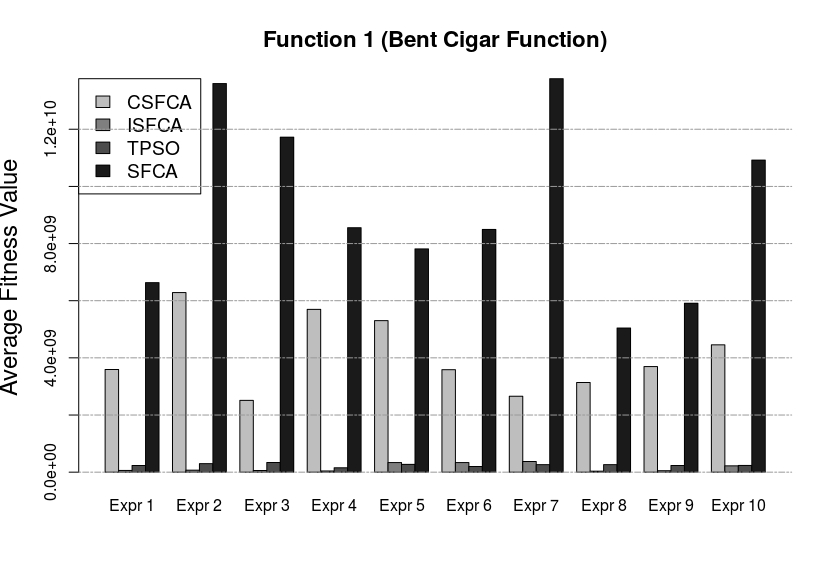
\includegraphics[scale=0.5]{func1_10}
	\centering
	\caption{Average fitness values for Function 1 with 10 dimensions}
	\label{func1_10}
\end{figure}
\begin{table}[H]
	\caption{function-1, dimension-30}
	\begin{tabular}{|c|c|c|c|c|}
		\hline
		& \textbf{SFPSO} & \textbf{CSFEP} & \textbf{SFEP} & \textbf{TPSO} \\ \hline
		\textbf{Median} & 1.224376E+10 & 9.035849E+09 & 3.381544E+10 & 1.223994E+10 \\ \hline
		\textbf{Mean} & 1.497176E+10 & 2.168689E+10 & 3.786293E+10 & 1.718683E+10 \\ \hline
		\textbf{Best} & 1.075684E+10 & 3.249525E+08 & 8.929425E+09 & 1.136511E+10 \\ \hline
		\textbf{StdDev} & 6.549615E+09 & 2.551255E+10 & 2.853221E+10 & 7.102879E+09 \\ \hline
	\end{tabular}
	\label{tbl1_30}
\end{table}
\begin{figure}[H]
	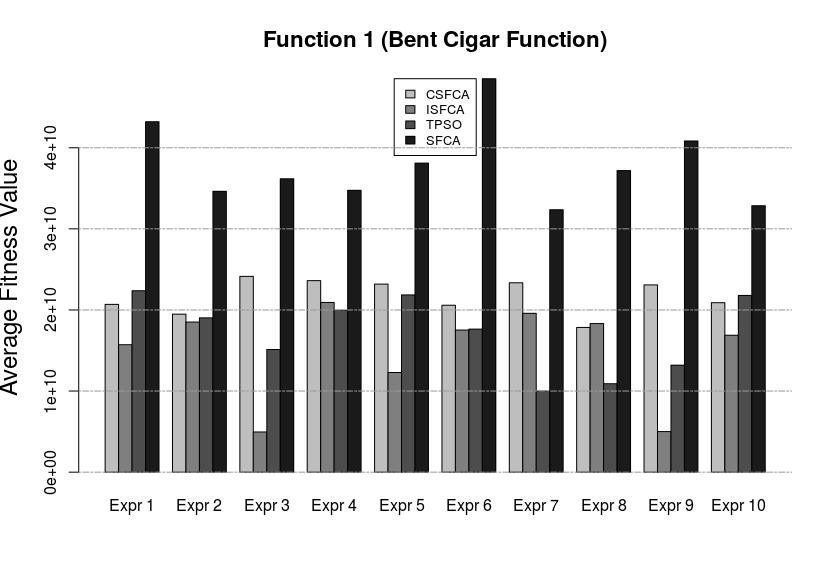
\includegraphics[scale=0.5]{func1_30}
	\centering
	\caption{Average fitness values for Function 1 with 30 dimensions}
	\label{func1_30}
\end{figure}

%\newpage

\section{Function 2: Discus Function}
As we can see in the table \ref{tbl2_10} and \ref{func2_10}, for 10-dimension optimization, ISFCA and CSFCA improve by 99\% and 42\% on the function 2. As explained in table \ref{tbl2_30} and \ref{func2_30}, they outperform the standard algorithm by 99\% and 95\% for 30-diemension optimization. 
\begin{table}[h]
	\caption{function-2, dimension-10}
	\begin{tabular}{|c|c|c|c|c|}
		\hline
		& \textbf{SFPSO} & \textbf{CSFEP} & \textbf{SFEP} & \textbf{TPSO} \\ \hline
		\textbf{Median} & 1.763602E+04 & 1.858882E+04 & 1.966669E+09 & 1.989622E+04 \\ \hline
		\textbf{Mean} & 1.970646E+04 & 2.045944E+09 & 3.574556E+09 & 2.202554E+04 \\ \hline
		\textbf{Best} & 1.690419E+04 & 1.426333E+04 & 2.467511E+04 & 1.722714E+04 \\ \hline
		\textbf{StdDev} & 5.285568E+03 & 4.083561E+09 & 4.508859E+09 & 5.505069E+03 \\ \hline
	\end{tabular}
	\label{tbl2_10}
\end{table}
\begin{figure}[h]
	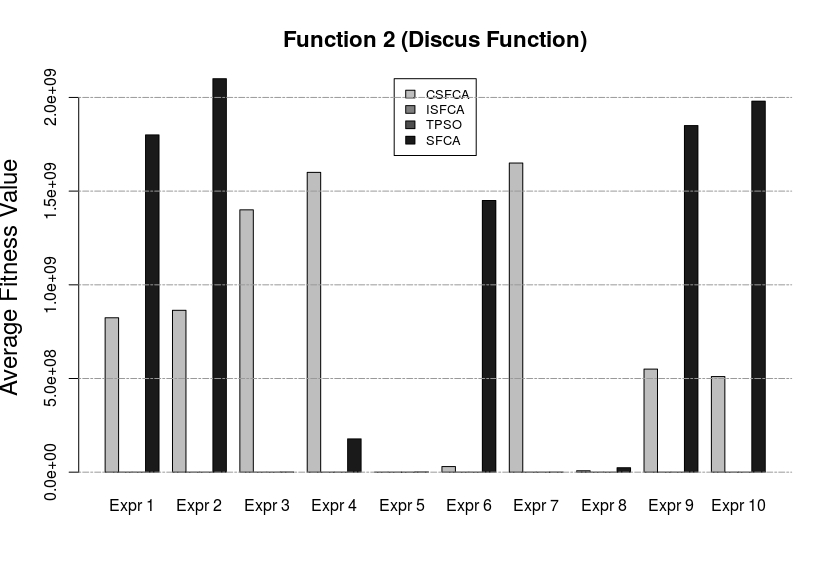
\includegraphics[scale=0.5]{func2_10}
	\centering
	\caption{Average fitness values for Function 2 with 10 dimensions}
	\label{func2_10}
\end{figure}
\begin{table}[h]
	\caption{function-2, dimension-30}
	\begin{tabular}{|c|c|c|c|c|}
		\hline
		& \textbf{SFPSO} & \textbf{CSFEP} & \textbf{SFEP} & \textbf{TPSO} \\ \hline
		\textbf{Median} & 7.057468E+04 & 6.106335E+04 & 8.669496E+07 & 1.338066E+05 \\ \hline
		\textbf{Mean} & 7.324758E+04 & 1.090201E+08 & 2.266584E+09 & 1.324195E+05 \\ \hline
		\textbf{Best} & 6.816396E+04 & 5.556673E+04 & 7.322705E+04 & 1.112664E+05 \\ \hline
		\textbf{StdDev} & 1.112414E+04 & 2.214664E+08 & 4.323029E+09 & 1.359207E+04 \\ \hline
	\end{tabular}
	\label{tbl2_30}
\end{table}
\begin{figure}[H]
	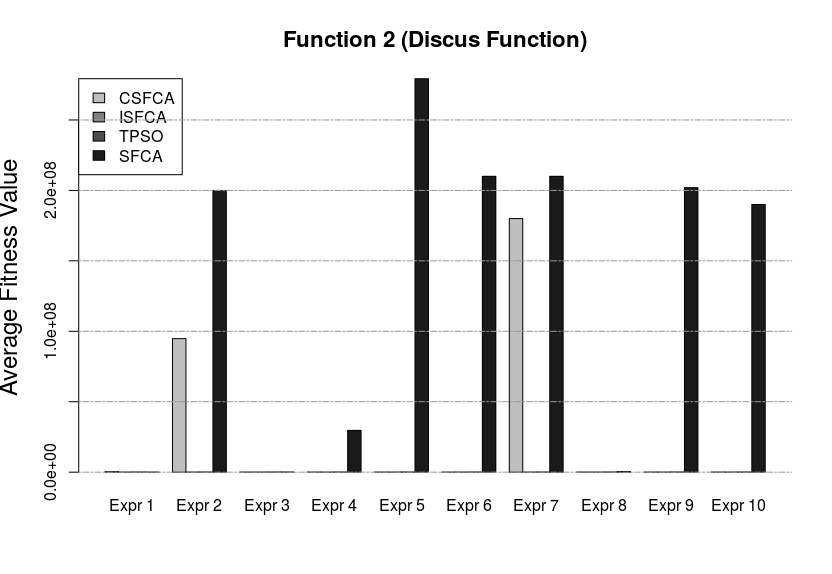
\includegraphics[scale=0.5]{func2_30}
	\centering
	\caption{Average fitness values for Function 2 with 30 dimensions}
	\label{func2_30}
\end{figure}

\section{Function 3: Weierstrass Function}
As you can see in Tables \ref{tbl3_10} and \ref{tbl3_30} and Figures \ref{func3_10} and \ref{func3_30}, the improvement of our approaches is trivial. However, it is still better than SFCA.
\begin{table}[h]
	\caption{function-3, dimension-10}
	\begin{tabular}{|c|c|c|c|c|}
		\hline
		& \textbf{SFPSO} & \textbf{CSFEP} & \textbf{SFEP} & \textbf{TPSO} \\ \hline
		\textbf{Median} & 3.053639E+02 & 3.088023E+02 & 3.106131E+02 & 3.059917E+02 \\ \hline
		\textbf{Mean} & 3.055362E+02 & 3.095236E+02 & 3.108567E+02 & 3.064904E+02 \\ \hline
		\textbf{Best} & 3.047026E+02 & 3.075572E+02 & 3.086619E+02 & 3.055813E+02 \\ \hline
		\textbf{StdDev} & 9.238688E-01 & 2.153735E+00 & 2.160320E+00 & 9.113892E-01 \\ \hline
	\end{tabular}
	\label{tbl3_10}
\end{table}

\begin{figure}[h]
	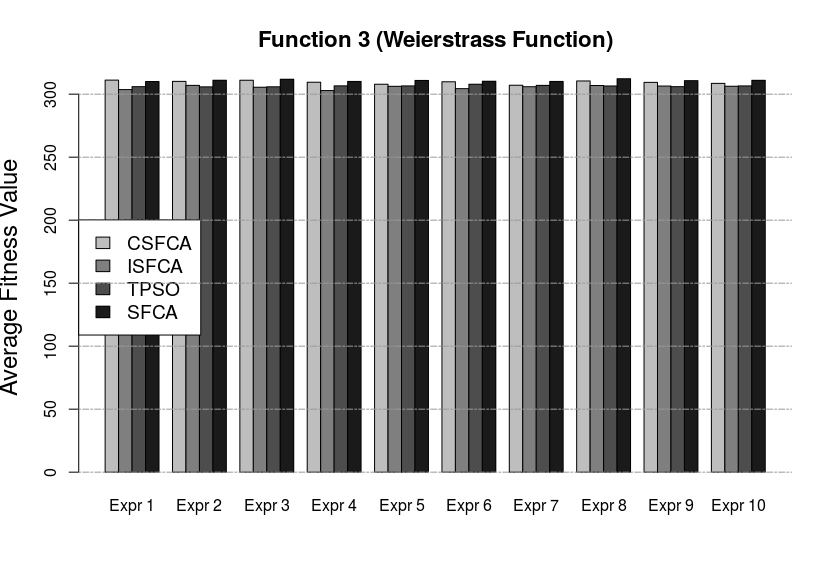
\includegraphics[scale=0.5]{func3_10}
	\centering
	\caption{Average fitness values for Function 3 with 10 dimensions}
	\label{func3_10}
\end{figure}

\begin{table}[h]
	\caption{function-3, dimension-30}
	\begin{tabular}{|c|c|c|c|c|}
		\hline
		& \textbf{SFPSO} & \textbf{CSFEP} & \textbf{SFEP} & \textbf{TPSO} \\ \hline
		\textbf{Median} & 3.288747E+02 & 3.395129E+02 & 3.414242E+02 & 3.276385E+02 \\ \hline
		\textbf{Mean} & 3.307785E+02 & 3.400480E+02 & 3.410312E+02 & 3.305742E+02 \\ \hline
		\textbf{Best} & 3.274619E+02 & 3.352212E+02 & 3.360418E+02 & 3.275333E+02 \\ \hline
		\textbf{StdDev} & 3.242337E+00 & 4.748334E+00 & 4.694844E+00 & 3.905358E+00 \\ \hline
	\end{tabular}
	\label{tbl3_30}
\end{table}
\begin{figure}[H]
	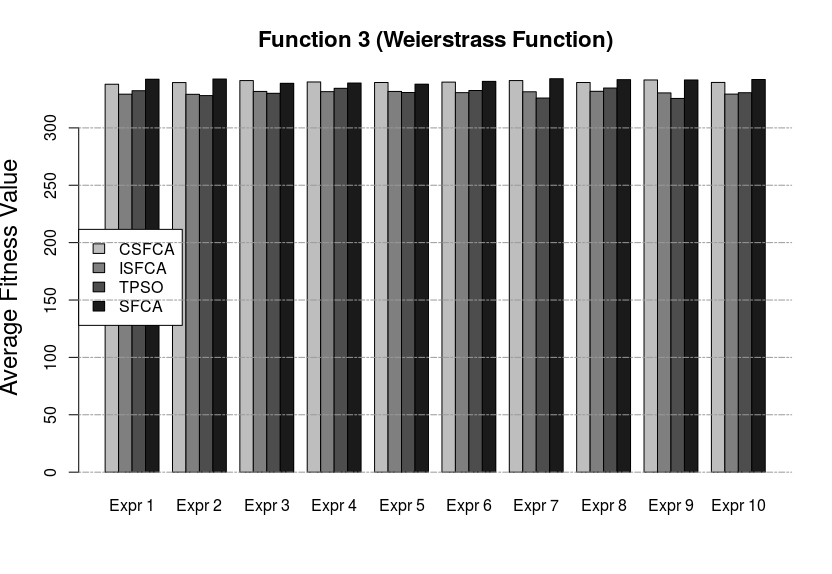
\includegraphics[scale=0.5]{func3_30}
	\centering
	\caption{Average fitness values for Function 3 with 30 dimensions}
	\label{func3_30}
\end{figure}

\section{Function 4: Modified Schwefel's Function}
Table \ref{tbl4_10} and figure \ref{func4_10} show that in the case 10-dimension optimizatoin, ISFCA performs better by 18\% and CSFCA by 19\%. However, for the 30-dimension case, only CSFCA outperform SFCA by 21\% as shown in Table \ref{tbl4_30} and Figure \ref{func4_30}.
\begin{table}[h]
	\caption{function-4, dimension-10}
	\begin{tabular}{|c|c|c|c|c|}
		\hline
		& \textbf{SFPSO} & \textbf{CSFEP} & \textbf{SFEP} & \textbf{TPSO} \\ \hline
		\textbf{Median} & 1.374025E+03 & 1.198259E+03 & 1.740208E+03 & 1.326440E+03 \\ \hline
		\textbf{Mean} & 1.401458E+03 & 1.392015E+03 & 1.725446E+03 & 1.391022E+03 \\ \hline
		\textbf{Best} & 1.249122E+03 & 6.135802E+02 & 8.405862E+02 & 1.201363E+03 \\ \hline
		\textbf{StdDev} & 1.709634E+02 & 8.047924E+02 & 8.388958E+02 & 2.174364E+02 \\ \hline
	\end{tabular}
	\label{tbl4_10}
\end{table}

\begin{figure}[h]
	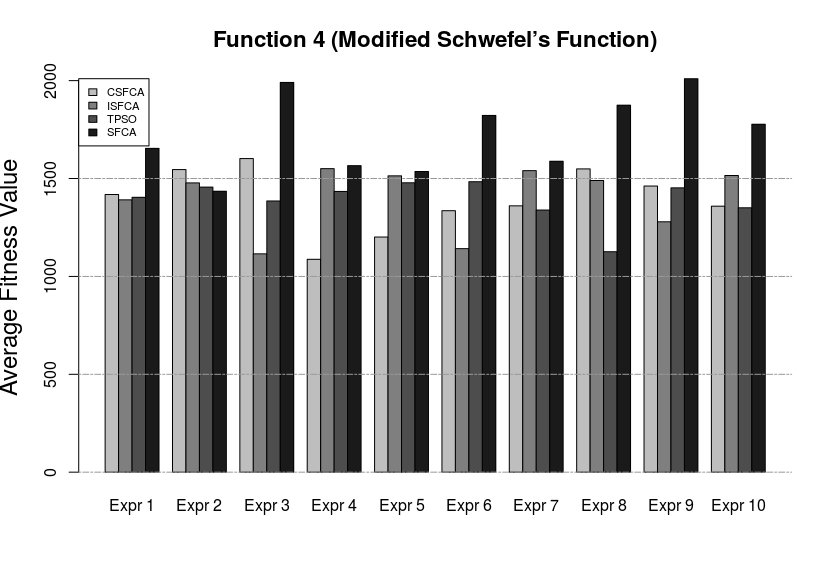
\includegraphics[scale=0.5]{func4_10}
	\centering
	\caption{Average fitness values for Function 4 with 10 dimensions}
	\label{func4_10}
\end{figure}

\begin{table}[h]
	\caption{function-4, dimension-30}
	\begin{tabular}{|c|c|c|c|c|}
		\hline
		& \textbf{SFPSO} & \textbf{CSFEP} & \textbf{SFEP} & \textbf{TPSO} \\ \hline
		\textbf{Median} & 6.870764E+03 & 5.098037E+03 & 6.819341E+03 & 7.117825E+03 \\ \hline
		\textbf{Mean} & 6.964474E+03 & 4.998230E+03 & 6.375121E+03 & 7.270199E+03 \\ \hline
		\textbf{Best} & 6.625647E+03 & 1.377132E+03 & 3.463489E+03 & 6.882440E+03 \\ \hline
		\textbf{StdDev} & 4.205720E+02 & 3.054933E+03 & 2.436783E+03 & 4.387157E+02 \\ \hline
	\end{tabular}
	\label{tbl4_30}
\end{table}

\begin{figure}[H]
	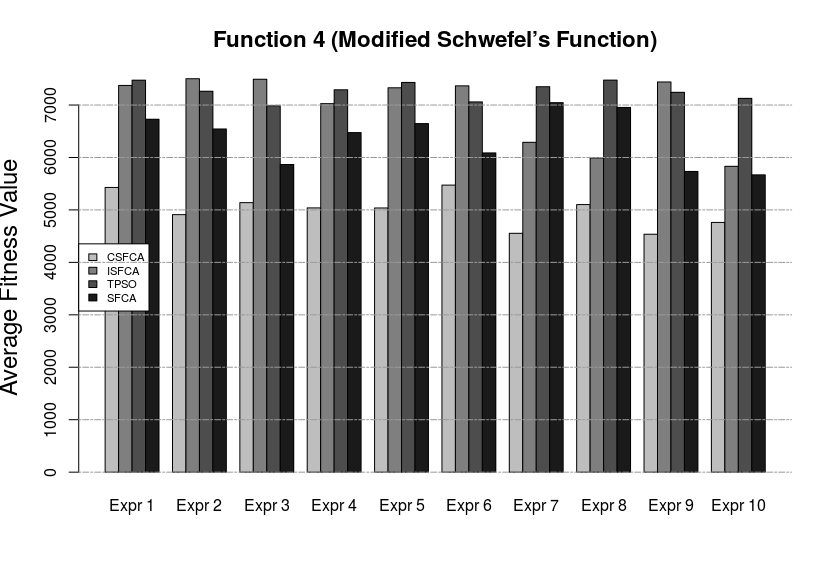
\includegraphics[scale=0.5]{func4_30}
	\centering
	\caption{Average fitness values for Function 4 with 30 dimensions}
	\label{func4_30}
\end{figure}

\section{Function 5: Katsuura Function}
As you can in Tables \ref{tbl5_10} and \ref{tbl5_30} and Figures \ref{func5_10} and \ref{func5_30}, the results of all the approaches are almost the same.
\begin{table}[h]
	\caption{function-5, dimension-10}
	\begin{tabular}{|c|c|c|c|c|}
		\hline
		& \textbf{SFPSO} & \textbf{CSFEP} & \textbf{SFEP} & \textbf{TPSO} \\ \hline
		\textbf{Median} & 5.012550E+02 & 5.014254E+02 & 5.019767E+02 & 5.012505E+02 \\ \hline
		\textbf{Mean} & 5.013300E+02 & 5.017117E+02 & 5.023857E+02 & 5.013223E+02 \\ \hline
		\textbf{Best} & 5.010726E+02 & 5.007002E+02 & 5.011836E+02 & 5.011289E+02 \\ \hline
		\textbf{StdDev} & 2.684750E-01 & 1.132619E+00 & 1.339239E+00 & 2.057213E-01 \\ \hline
	\end{tabular}
	\label{tbl5_10}
\end{table}

\begin{figure}[h]
	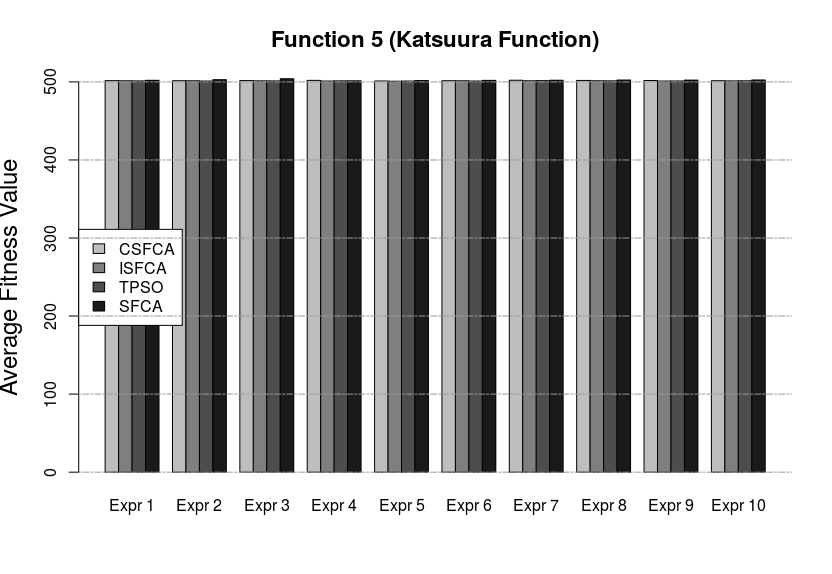
\includegraphics[scale=0.5]{func5_10}
	\centering
	\caption{Average fitness values for Function 5 with 10 dimensions}
	\label{func5_10}
\end{figure}

\begin{table}[h]
	\caption{function-5, dimension-30}
	\begin{tabular}{|c|c|c|c|c|}
		\hline
		& \textbf{SFPSO} & \textbf{CSFEP} & \textbf{SFEP} & \textbf{TPSO} \\ \hline
		\textbf{Median} & 5.029073E+02 & 5.025217E+02 & 5.030453E+02 & 5.028359E+02 \\ \hline
		\textbf{Mean} & 5.030805E+02 & 5.031380E+02 & 5.036162E+02 & 5.029678E+02 \\ \hline
		\textbf{Best} & 5.028153E+02 & 5.016618E+02 & 5.020560E+02 & 5.026209E+02 \\ \hline
		\textbf{StdDev} & 3.548877E-01 & 1.669277E+00 & 1.678840E+00 & 3.015601E-01 \\ \hline
	\end{tabular}
	\label{tbl5_30}
\end{table}
\begin{figure}[H]
	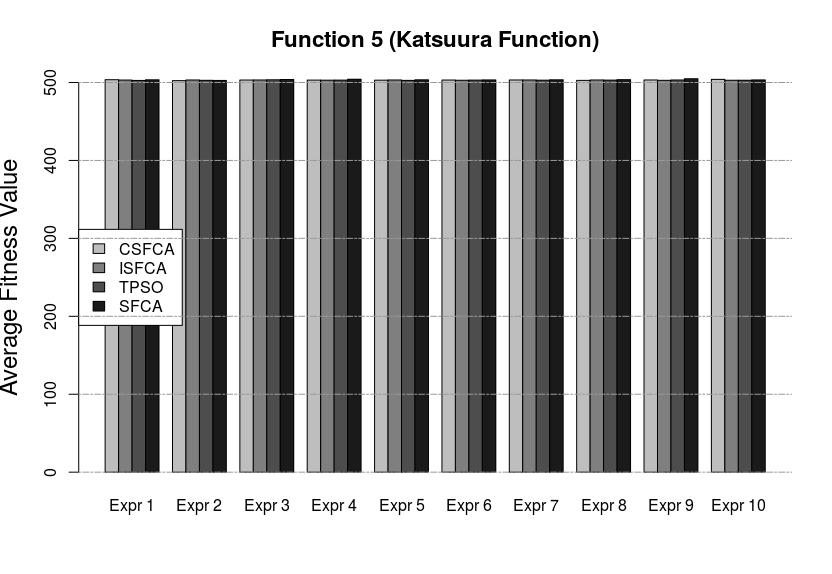
\includegraphics[scale=0.5]{func5_30}
	\centering
	\caption{Average fitness values for Function 5 with 30 dimensions}
	\label{func5_30}
\end{figure}

\newpage

\section{Function 6: HappyCat Function}
As you can see in Tables \ref{tbl6_10} and \ref{tbl6_30} and Figures \ref{func6_10} and \ref{func6_10}, the improvement of our approaches is trivial.
\begin{table}[h]
	\caption{function-6, dimension-10}
	\begin{tabular}{|c|c|c|c|c|}
		\hline
		& \textbf{SFPSO} & \textbf{CSFEP} & \textbf{SFEP} & \textbf{TPSO} \\ \hline
		\textbf{Median} & 6.004688E+02 & 6.015392E+02 & 6.033087E+02 & 6.005062E+02 \\ \hline
		\textbf{Mean} & 6.005623E+02 & 6.025225E+02 & 6.036813E+02 & 6.009515E+02 \\ \hline
		\textbf{Best} & 6.004334E+02 & 6.005685E+02 & 6.018524E+02 & 6.005062E+02 \\ \hline
		\textbf{StdDev} & 3.200289E-01 & 2.304279E+00 & 1.898523E+00 & 6.229300E-01 \\ \hline
	\end{tabular}
	\label{tbl6_10}
\end{table}

\begin{figure}[h]
	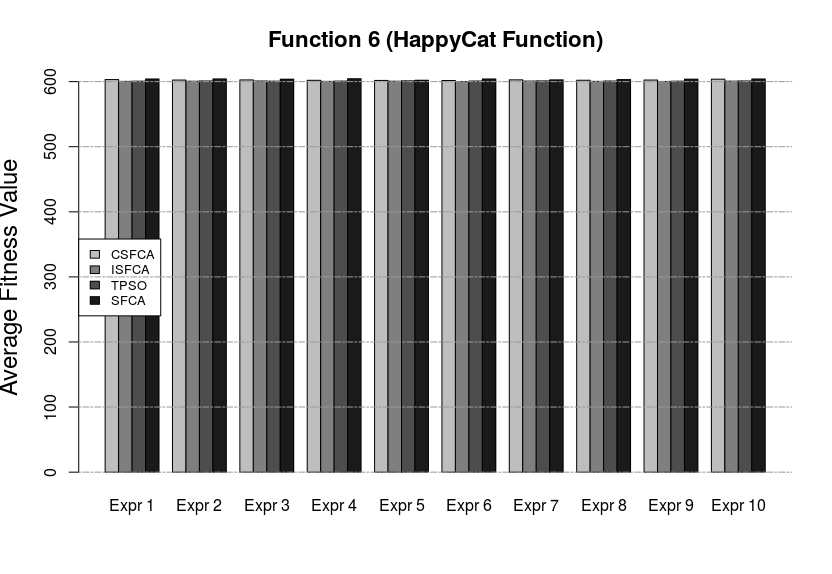
\includegraphics[scale=0.5]{func6_10}
	\centering
	\caption{Average fitness values for Function 6 with 10 dimensions}
	\label{func6_10}
\end{figure}

\begin{table}[h]
	\caption{function-6, dimension-30}
	\begin{tabular}{|c|c|c|c|c|}
		\hline
		& \textbf{SFPSO} & \textbf{CSFEP} & \textbf{SFEP} & \textbf{TPSO} \\ \hline
		\textbf{Median} & 6.025572E+02 & 6.038615E+02 & 6.054925E+02 & 6.010077E+02 \\ \hline
		\textbf{Mean} & 6.030236E+02 & 6.039768E+02 & 6.056628E+02 & 6.019309E+02 \\ \hline
		\textbf{Best} & 6.024192E+02 & 6.010681E+02 & 6.041570E+02 & 6.010077E+02 \\ \hline
		\textbf{StdDev} & 7.579661E-01 & 2.740738E+00 & 1.433152E+00 & 1.224478E+00 \\ \hline
	\end{tabular}
	\label{tbl6_30}
\end{table}
\begin{figure}[H]
	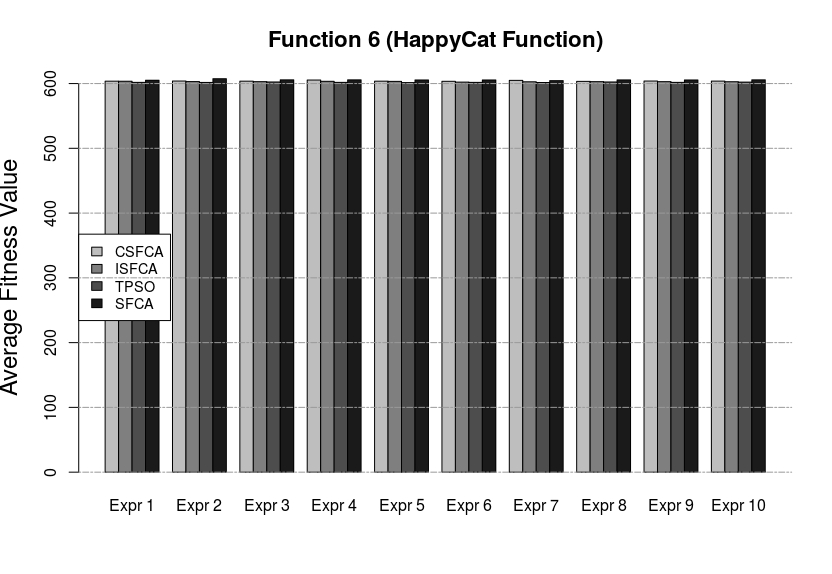
\includegraphics[scale=0.5]{func6_30}
	\centering
	\caption{Average fitness values for Function 6 with 30 dimensions}
	\label{func6_30}
\end{figure}

\newpage

\section{Function 7: HGBat Function}
As you can see in Tables \ref{tbl7_10} and \ref{tbl7_30} and Figures \ref{func7_10} and \ref{func7_10}, the improvement of our approaches is not so much. In the case of 10-dimension optimization, it is about 5\% and for the 30-dimension case, it is about 9\%. 
\begin{table}[h]
	\caption{function-7, dimension-10}
	\begin{tabular}{|c|c|c|c|c|}
		\hline
		& \textbf{SFPSO} & \textbf{CSFEP} & \textbf{SFEP} & \textbf{TPSO} \\ \hline
		\textbf{Median} & 7.008041E+02 & 7.081532E+02 & 7.341129E+02 & 7.004902E+02 \\ \hline
		\textbf{Mean} & 7.019942E+02 & 7.260979E+02 & 7.418000E+02 & 7.038384E+02 \\ \hline
		\textbf{Best} & 7.006188E+02 & 7.007965E+02 & 7.100632E+02 & 7.004902E+02 \\ \hline
		\textbf{StdDev} & 2.635216E+00 & 3.539268E+01 & 3.490056E+01 & 5.486938E+00 \\ \hline
	\end{tabular}
	\label{tbl7_10}
\end{table}

\begin{figure}[h]
	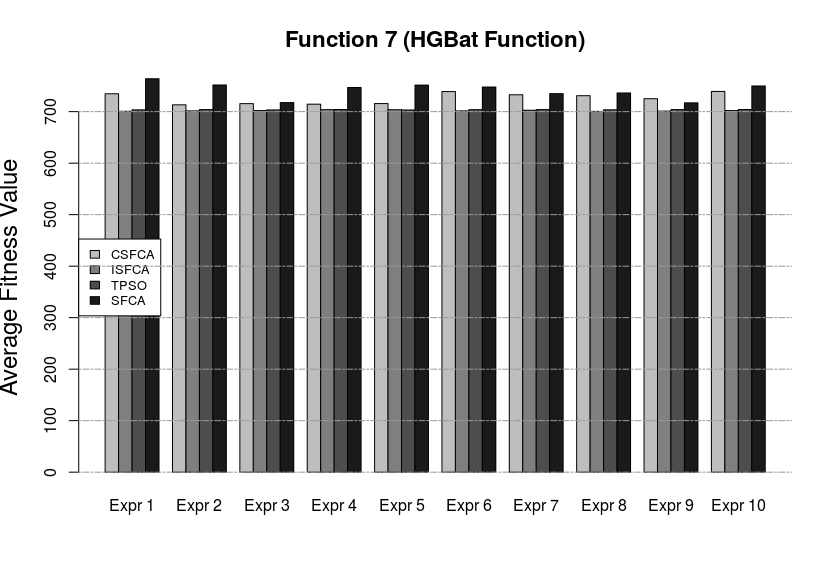
\includegraphics[scale=0.5]{func7_10}
	\centering
	\caption{Average fitness values for Function 7 with 10 dimensions}
	\label{func7_10}
\end{figure}

\begin{table}[h]
	\caption{function-7, dimension-30}
	\begin{tabular}{|c|c|c|c|c|}
		\hline
		& \textbf{SFPSO} & \textbf{CSFEP} & \textbf{SFEP} & \textbf{TPSO} \\ \hline
		\textbf{Median} & 7.291294E+02 & 7.477774E+02 & 8.042494E+02 & 7.280204E+02 \\ \hline
		\textbf{Mean} & 7.389013E+02 & 7.605963E+02 & 8.116680E+02 & 7.498652E+02 \\ \hline
		\textbf{Best} & 7.271223E+02 & 7.024000E+02 & 7.544377E+02 & 7.262179E+02 \\ \hline
		\textbf{StdDev} & 1.569694E+01 & 5.981939E+01 & 5.740507E+01 & 2.791729E+01 \\ \hline
	\end{tabular}
	\label{tbl7_30}
\end{table}
\begin{figure}[H]
	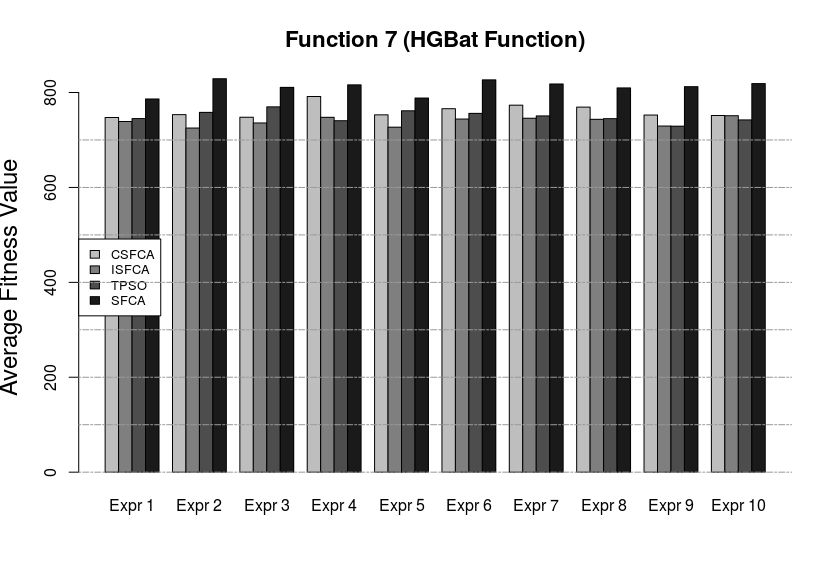
\includegraphics[scale=0.5]{func7_30}
	\centering
	\caption{Average fitness values for Function 7 with 30 dimensions}
	\label{func7_30}
\end{figure}

\section{Function 8: Griewank's plus Rosenbrock's Function}
In table \ref{tbl8_10} and figure \ref{func8_10}, we can see that both of our approaches (ISFCA and CSFCA) and TPSO outperform the standard SFCA impressively with 99\% and 77\% for optimization of 10 dimensions. In the case of 30-dimension optimization, ISFCA and CSFCA perform with 97\% and 52\% improvement respectively as shown in Table \ref{tbl8_30} and Figure \ref{func8_30}. 
\begin{table}[h]
	\caption{function-8, dimension-10}
	\begin{tabular}{|c|c|c|c|c|}
		\hline
		& \textbf{SFPSO} & \textbf{CSFEP} & \textbf{SFEP} & \textbf{TPSO} \\ \hline
		\textbf{Median} & 8.060488E+02 & 4.762535E+03 & 5.638811E+05 & 8.057399E+02 \\ \hline
		\textbf{Mean} & 8.327824E+02 & 3.080861E+05 & 1.374142E+06 & 8.319941E+02 \\ \hline
		\textbf{Best} & 8.060488E+02 & 8.475602E+02 & 4.118304E+03 & 8.057399E+02 \\ \hline
		\textbf{StdDev} & 1.428379E+02 & 5.970746E+05 & 1.940514E+06 & 7.254239E+01 \\ \hline
	\end{tabular}
	\label{tbl8_10}
\end{table}

\begin{figure}[h]
	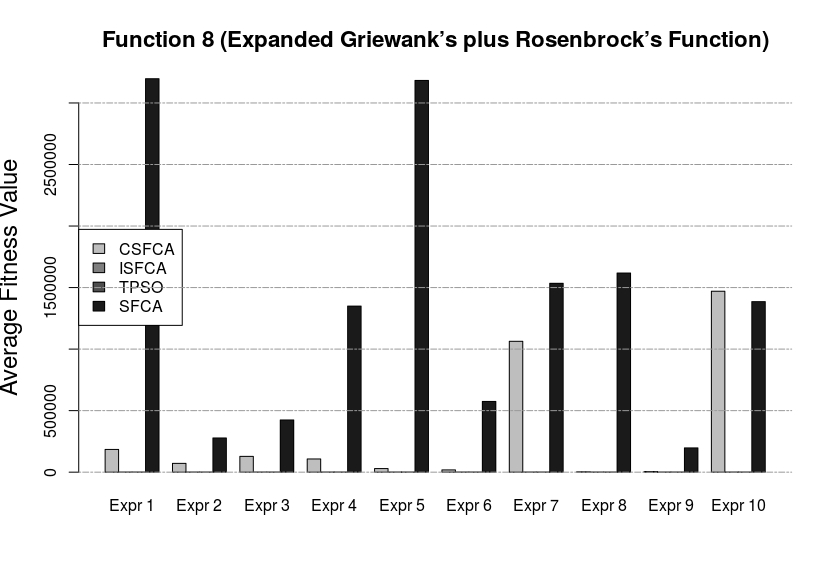
\includegraphics[scale=0.5]{func8_10}
	\centering
	\caption{Average fitness values for Function 8 with 10 dimensions}
	\label{func8_10}
\end{figure}

\begin{table}[h]
	\caption{function-8, dimension-30}
	\begin{tabular}{|c|c|c|c|c|}
		\hline
		& \textbf{SFPSO} & \textbf{CSFEP} & \textbf{SFEP} & \textbf{TPSO} \\ \hline
		\textbf{Median} & 1.139271E+05 & 3.872060E+05 & 3.562129E+06 & 8.406430E+05 \\ \hline
		\textbf{Mean} & 3.363145E+05 & 7.477703E+06 & 1.541796E+07 & 1.645666E+06 \\ \hline
		\textbf{Best} & 5.240269E+04 & 1.095824E+03 & 8.508643E+04 & 4.126489E+05 \\ \hline
		\textbf{StdDev} & 6.891847E+05 & 1.270040E+07 & 2.340250E+07 & 1.667678E+06 \\ \hline
	\end{tabular}
	\label{tbl8_30}
\end{table}
\begin{figure}[H]
	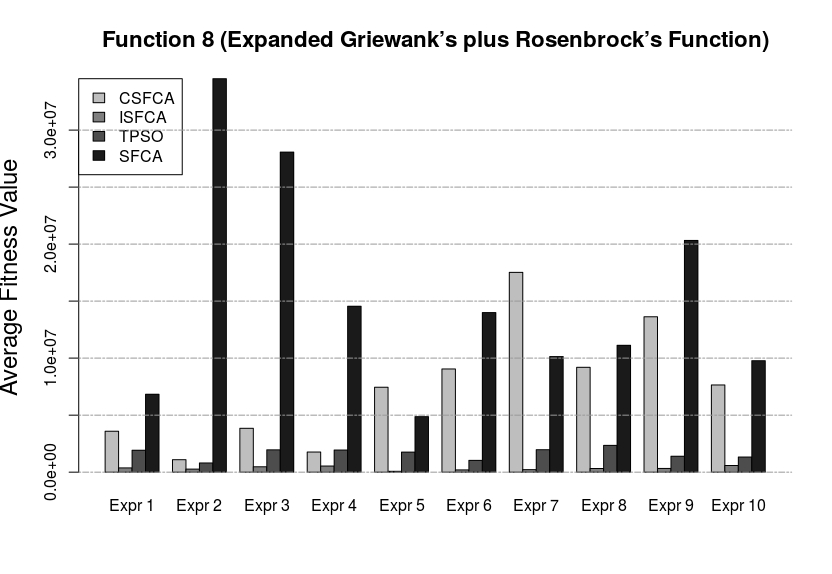
\includegraphics[scale=0.5]{func8_30}
	\centering
	\caption{Average fitness values for Function 8 with 30 dimensions}
	\label{func8_30}
\end{figure}

\section{Function 9: Expanded Scaffer's F6 Function}
In Tables \ref{tbl9_10} and \ref{tbl9_30} and Figures \ref{func9_10} and \ref{func9_30}, we can see that there is not a considerable improvement and all the methods perform almost the same.
\begin{table}[h]
	\caption{function-9, dimension-10}
	\begin{tabular}{|c|c|c|c|c|}
		\hline
		& \textbf{SFPSO} & \textbf{CSFEP} & \textbf{SFEP} & \textbf{TPSO} \\ \hline
		\textbf{Median} & 9.036094E+02 & 9.035775E+02 & 9.037811E+02 & 9.035661E+02 \\ \hline
		\textbf{Mean} & 9.036469E+02 & 9.036343E+02 & 9.038043E+02 & 9.036178E+02 \\ \hline
		\textbf{Best} & 9.035325E+02 & 9.032589E+02 & 9.033602E+02 & 9.035094E+02 \\ \hline
		\textbf{StdDev} & 1.008688E-01 & 3.372815E-01 & 4.187602E-01 & 1.037992E-01 \\ \hline
	\end{tabular}
	\label{tbl9_10}
\end{table}

\begin{figure}[h]
	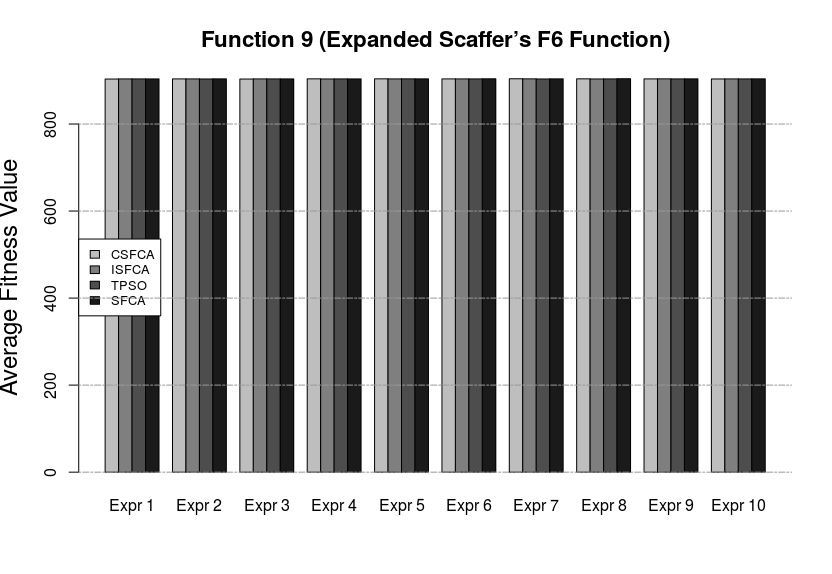
\includegraphics[scale=0.5]{func9_10}
	\centering
	\caption{Average fitness values for Function 9 with 10 dimensions}
	\label{func9_10}
\end{figure}

\begin{table}[h]
	\caption{function-9, dimension-30}
	\begin{tabular}{|c|c|c|c|c|}
		\hline
		& \textbf{SFPSO} & \textbf{CSFEP} & \textbf{SFEP} & \textbf{TPSO} \\ \hline
		\textbf{Median} & 9.134898E+02 & 9.134569E+02 & 9.136834E+02 & 9.135212E+02 \\ \hline
		\textbf{Mean} & 9.135258E+02 & 9.133575E+02 & 9.136351E+02 & 9.135977E+02 \\ \hline
		\textbf{Best} & 9.133757E+02 & 9.126562E+02 & 9.131192E+02 & 9.134243E+02 \\ \hline
		\textbf{StdDev} & 1.312660E-01 & 5.882330E-01 & 4.913793E-01 & 1.390313E-01 \\ \hline
	\end{tabular}
	\label{tbl9_30}
\end{table}
\begin{figure}[H]
	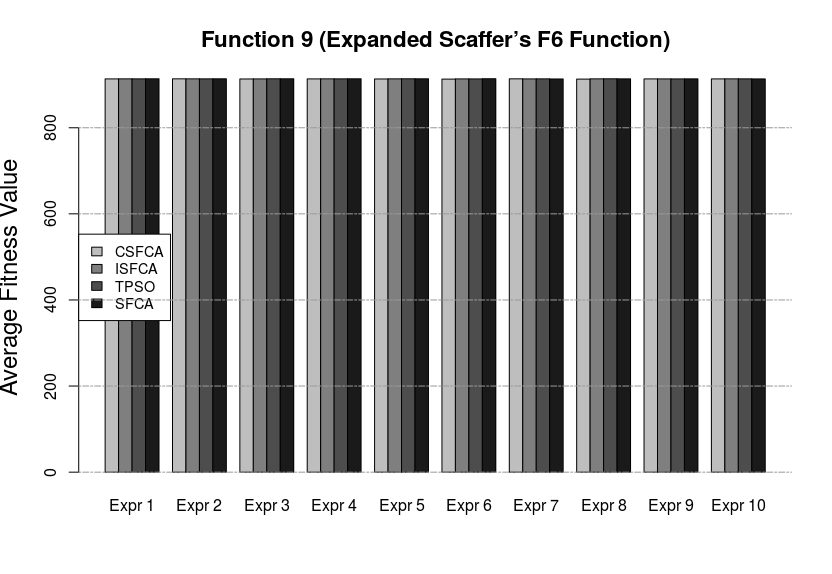
\includegraphics[scale=0.5]{func9_30}
	\centering
	\caption{Average fitness values for Function 9 with 30 dimensions}
	\label{func9_30}
\end{figure}

\section{Function 10: Hybrid Function 1}
In the 10-dimension case, Table \ref{tbl10_10} and Figure \ref{func10_10} show an impressive improvement for both ISFCA and CSFCA approaches by 99\% and 77\% respectively. For the 30-dimension case, ISFCA and CSFCA outperform SFCA by 97\% and 51\% respectively as shown in Table \ref{tbl10_30} and Figure \ref{func10_30}.
\begin{table}[h]
	\caption{function-10, dimension-10}
	\begin{tabular}{|c|c|c|c|c|}
		\hline
		& \textbf{SFPSO} & \textbf{CSFEP} & \textbf{SFEP} & \textbf{TPSO} \\ \hline
		\textbf{Median} & 5.078678E+04 & 5.565684E+05 & 1.462417E+06 & 3.479607E+04 \\ \hline
		\textbf{Mean} & 6.855882E+04 & 1.390710E+06 & 1.250589E+07 & 6.576307E+04 \\ \hline
		\textbf{Best} & 2.148022E+04 & 2.365329E+03 & 6.578523E+03 & 1.417589E+04 \\ \hline
		\textbf{StdDev} & 7.234730E+04 & 1.778552E+06 & 2.276703E+07 & 7.783437E+04 \\ \hline
	\end{tabular}
	\label{tbl10_10}
\end{table}

\begin{figure}[h]
	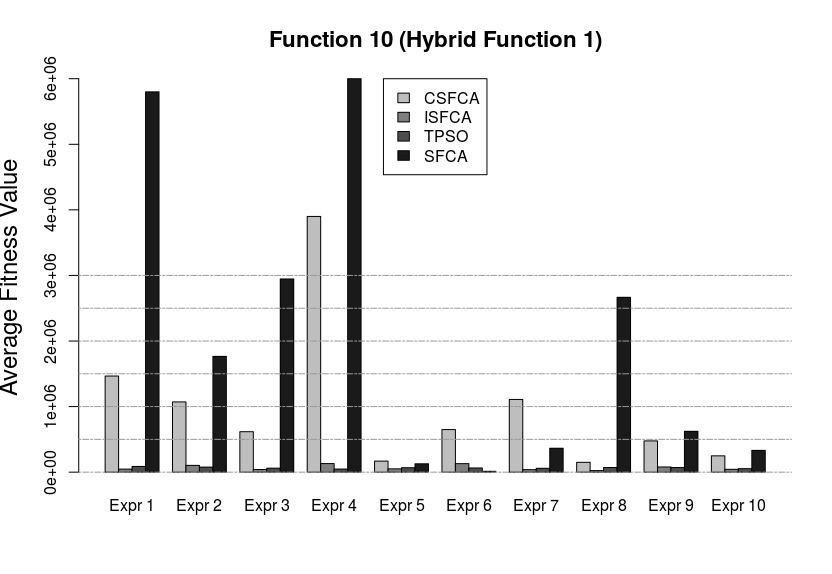
\includegraphics[scale=0.5]{func10_10}
	\centering
	\caption{Average fitness values for Function 10 with 10 dimensions}
	\label{func10_10}
\end{figure}

\begin{table}[h]
	\caption{function-10, dimension-30}
	\begin{tabular}{|c|c|c|c|c|}
		\hline
		& \textbf{SFPSO} & \textbf{CSFEP} & \textbf{SFEP} & \textbf{TPSO} \\ \hline
		\textbf{Median} & 1.257686E+07 & 2.886032E+07 & 7.068932E+07 & 1.524856E+07 \\ \hline
		\textbf{Mean} & 1.288355E+07 & 5.268560E+07 & 7.171894E+07 & 1.914266E+07 \\ \hline
		\textbf{Best} & 6.072906E+06 & 2.225892E+06 & 8.682100E+06 & 1.311979E+07 \\ \hline
		\textbf{StdDev} & 7.703664E+06 & 5.803312E+07 & 5.952516E+07 & 8.464172E+06 \\ \hline
	\end{tabular}
	\label{tbl10_30}
\end{table}
\begin{figure}[H]
	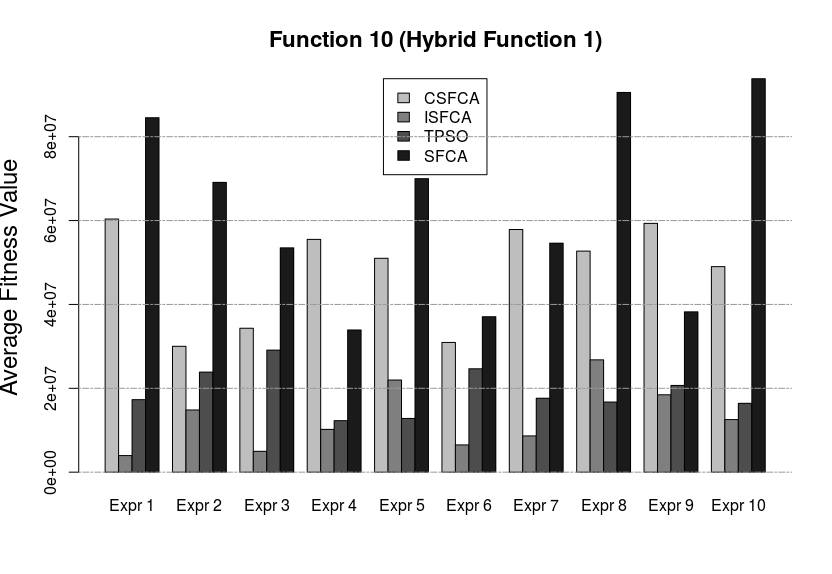
\includegraphics[scale=0.5]{func10_30}
	\centering
	\caption{Average fitness values for Function 10 with 30 dimensions}
	\label{func10_30}
\end{figure}

\section{Function 11: Hybrid Function 2}
 Table \ref{tbl11_10} and Figure \ref{func11_10} show a trivial improvement for the 10-dimension case. On the other hand, Table \ref{tbl11_30} and Figure \ref{func11_30} explain that ISFCA and CSFCA outperform the standard algorithm by 30\% and 15\% respectively.
\begin{table}[h]
	\caption{function-11, dimension-10}
	\begin{tabular}{|c|c|c|c|c|}
		\hline
		& \textbf{SFPSO} & \textbf{CSFEP} & \textbf{SFEP} & \textbf{TPSO} \\ \hline
		\textbf{Median} & 1.104725E+03 & 1.109982E+03 & 1.111399E+03 & 1.104917E+03 \\ \hline
		\textbf{Mean} & 1.105085E+03 & 1.137076E+03 & 1.140188E+03 & 1.105442E+03 \\ \hline
		\textbf{Best} & 1.104062E+03 & 1.106581E+03 & 1.105492E+03 & 1.104723E+03 \\ \hline
		\textbf{StdDev} & 1.339530E+00 & 5.229237E+01 & 4.994351E+01 & 9.340507E-01 \\ \hline
	\end{tabular}
	\label{tbl11_10}
\end{table}

\begin{figure}[h]
	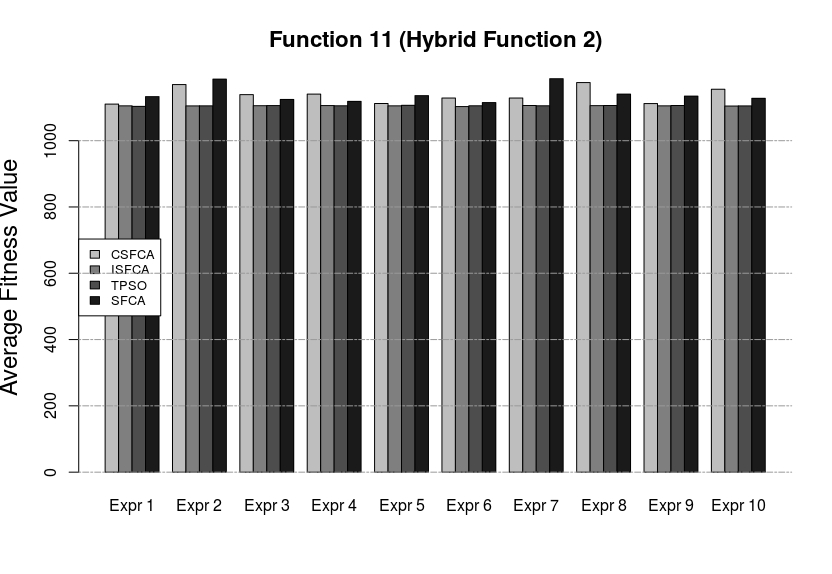
\includegraphics[scale=0.5]{func11_10}
	\centering
	\caption{Average fitness values for Function 11 with 10 dimensions}
	\label{func11_10}
\end{figure}

\begin{table}[h]
	\caption{function-11, dimension-30}
	\begin{tabular}{|c|c|c|c|c|}
		\hline
		& \textbf{SFPSO} & \textbf{CSFEP} & \textbf{SFEP} & \textbf{TPSO} \\ \hline
		\textbf{Median} & 1.188478E+03 & 1.246676E+03 & 1.561269E+03 & 1.134562E+03 \\ \hline
		\textbf{Mean} & 1.197912E+03 & 1.456495E+03 & 1.724513E+03 & 1.174516E+03 \\ \hline
		\textbf{Best} & 1.153360E+03 & 1.155965E+03 & 1.290852E+03 & 1.134562E+03 \\ \hline
		\textbf{StdDev} & 4.334944E+01 & 4.589486E+02 & 5.277303E+02 & 6.235017E+01 \\ \hline
	\end{tabular}
	\label{tbl11_30}
\end{table}
\begin{figure}[H]
	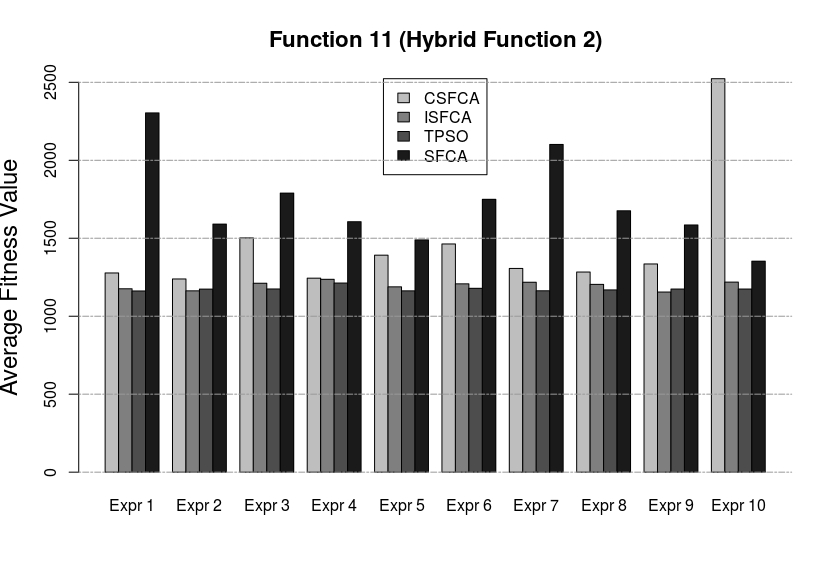
\includegraphics[scale=0.5]{func11_30}
	\centering
	\caption{Average fitness values for Function 11 with 30 dimensions}
	\label{func11_30}
\end{figure}

\section{Function 12: Hybrid Function 3}
Both of ISFCA and CSFCA approaches perform much better than the standard algorithm in both 10-dimension and 30-dimension scenarios. Table \ref{tbl12_10} and Figure \ref{func12_10} show that ISFCA and CSFCA improve the performance by 93\% and 82\% for the 10-dimension case. Table \ref{tbl12_30} and Figure \ref{func12_30} indicate that ISFCA and CSFCA improve the peformance by 99\% and 68\% for the 30-dimension case.
\begin{table}[h]
	\caption{function-12, dimension-10}
	\begin{tabular}{|c|c|c|c|c|}
		\hline
		& \textbf{SFPSO} & \textbf{CSFEP} & \textbf{SFEP} & \textbf{TPSO} \\ \hline
		\textbf{Median} & 1.278429E+03 & 1.470304E+03 & 2.561160E+03 & 1.274117E+03 \\ \hline
		\textbf{Mean} & 1.284340E+03 & 3.740383E+03 & 2.109208E+04 & 1.290392E+03 \\ \hline
		\textbf{Best} & 1.247398E+03 & 1.342194E+03 & 1.419410E+03 & 1.259420E+03 \\ \hline
		\textbf{StdDev} & 4.080435E+01 & 4.569942E+03 & 3.705284E+04 & 4.016558E+01 \\ \hline
	\end{tabular}
	\label{tbl12_10}
\end{table}

\begin{figure}[h]
	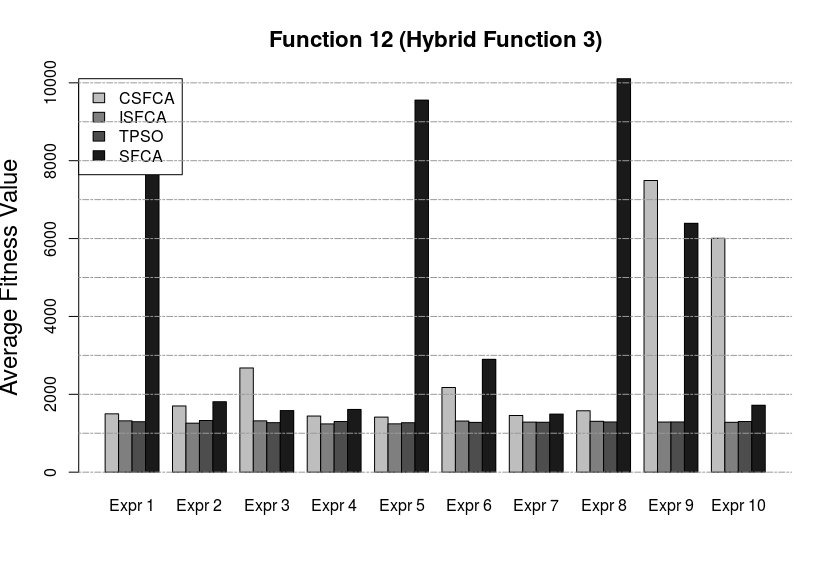
\includegraphics[scale=0.5]{func12_10}
	\centering
	\caption{Average fitness values for Function 12 with 10 dimensions}
	\label{func12_10}
\end{figure}

\begin{table}[h]
	\caption{function-12, dimension-30}
	\begin{tabular}{|c|c|c|c|c|}
		\hline
		& \textbf{SFPSO} & \textbf{CSFEP} & \textbf{SFEP} & \textbf{TPSO} \\ \hline
		\textbf{Median} & 2.262814E+03 & 2.093796E+03 & 8.098215E+07 & 2.280177E+03 \\ \hline
		\textbf{Mean} & 2.317707E+03 & 3.578488E+07 & 1.123866E+08 & 2.392247E+03 \\ \hline
		\textbf{Best} & 2.100877E+03 & 1.748342E+03 & 2.153439E+03 & 2.280177E+03 \\ \hline
		\textbf{StdDev} & 2.430944E+02 & 7.154759E+07 & 1.253791E+08 & 1.588321E+02 \\ \hline
	\end{tabular}
	\label{tbl12_30}
\end{table}
\begin{figure}[H]
	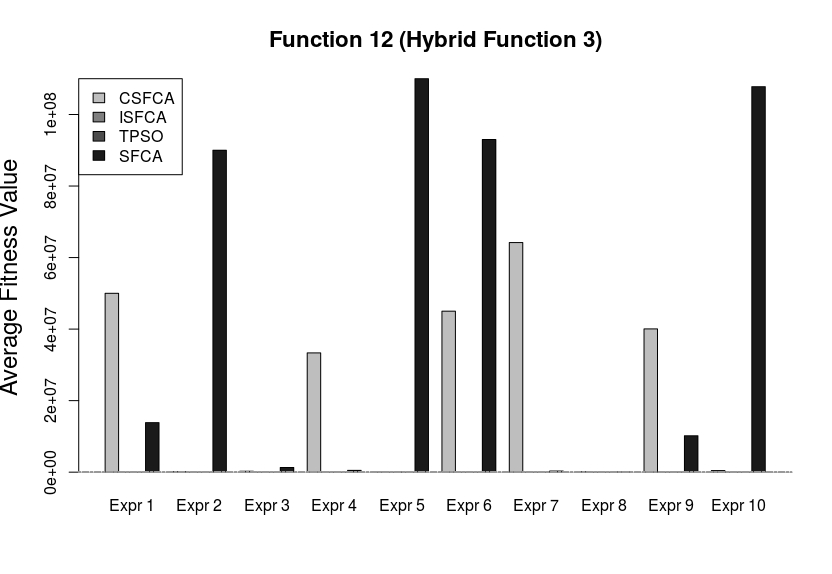
\includegraphics[scale=0.5]{func12_30}
	\centering
	\caption{Average fitness values for Function 12 with 30 dimensions}
	\label{func12_30}
\end{figure}

\section{Function 13: Composition Function 1}
This function is improved moderately in both 10- and 30-diemnsion cases. Table \ref{tbl13_10} and Figure \ref{func13_10} show that ISFCA and CSFCA improve the average fitness values for the 10-dimension case by 31\% and 10\% respectively. For the 30-dimension case, in Table \ref{tbl13_30} and \ref{func13_30}, we can see that ISFCA and CSFCA improve the performance by 51\% and 6\% respectively.
\begin{table}[h]
	\caption{function-13, dimension-10}
	\begin{tabular}{|c|c|c|c|c|}
		\hline
		& \textbf{SFPSO} & \textbf{CSFEP} & \textbf{SFEP} & \textbf{TPSO} \\ \hline
		\textbf{Median} & 1.626676E+03 & 1.750040E+03 & 2.101426E+03 & 1.623272E+03 \\ \hline
		\textbf{Mean} & 1.627982E+03 & 2.128914E+03 & 2.376883E+03 & 1.628781E+03 \\ \hline
		\textbf{Best} & 1.622335E+03 & 1.635087E+03 & 1.676418E+03 & 1.618919E+03 \\ \hline
		\textbf{StdDev} & 7.106025E+00 & 6.591729E+02 & 7.972695E+02 & 1.445686E+01 \\ \hline
	\end{tabular}
	\label{tbl13_10}
\end{table}

\begin{figure}[h]
	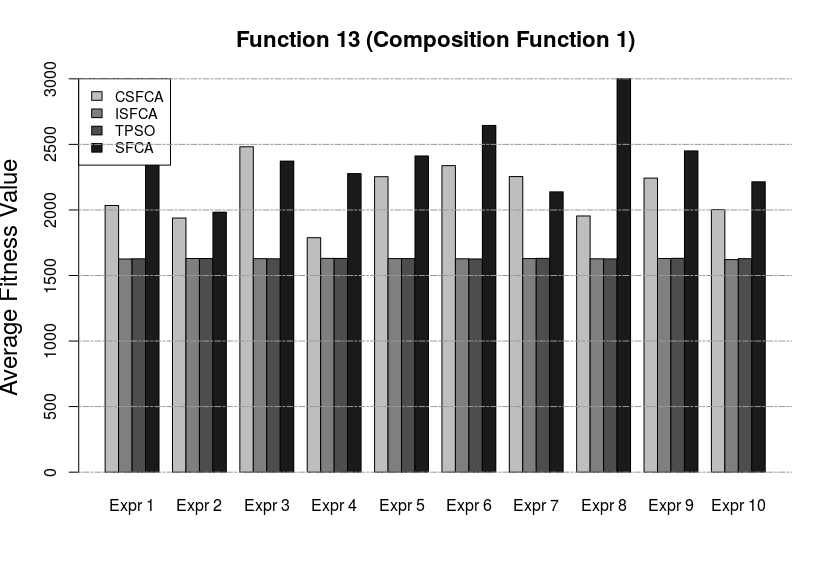
\includegraphics[scale=0.5]{func13_10}
	\centering
	\caption{Average fitness values for Function 13 with 10 dimensions}
	\label{func13_10}
\end{figure}

\begin{table}[h]
	\caption{function-13, dimension-30}
	\begin{tabular}{|c|c|c|c|c|}
		\hline
		& \textbf{SFPSO} & \textbf{CSFEP} & \textbf{SFEP} & \textbf{TPSO} \\ \hline
		\textbf{Median} & 1.727952E+03 & 2.442454E+03 & 3.419566E+03 & 1.742700E+03 \\ \hline
		\textbf{Mean} & 1.778258E+03 & 3.445463E+03 & 3.691270E+03 & 1.840829E+03 \\ \hline
		\textbf{Best} & 1.723534E+03 & 1.740536E+03 & 2.380543E+03 & 1.732389E+03 \\ \hline
		\textbf{StdDev} & 9.665278E+01 & 2.272010E+03 & 1.367277E+03 & 1.457157E+02 \\ \hline
	\end{tabular}
	\label{tbl13_30}
\end{table}
\begin{figure}[H]
	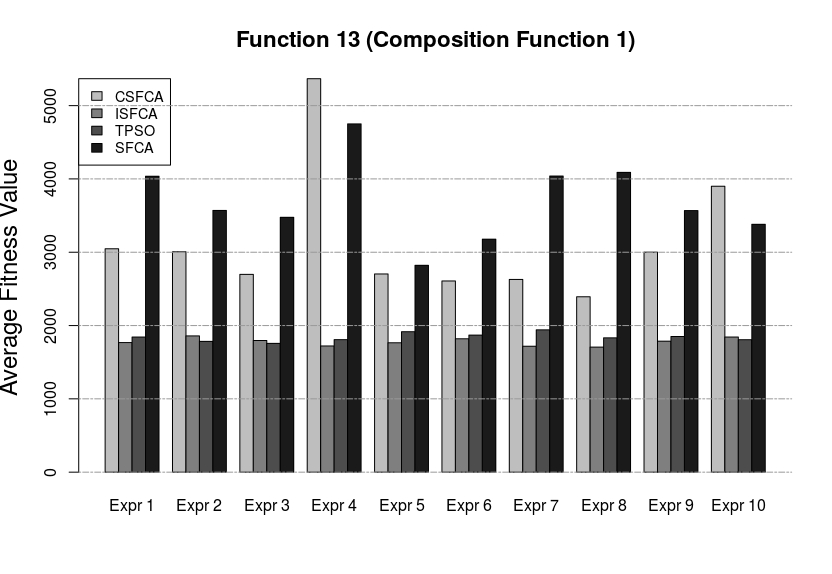
\includegraphics[scale=0.5]{func13_30}
	\centering
	\caption{Average fitness values for Function 13 with 30 dimensions}
	\label{func13_30}
\end{figure}

\section{Function 14: Composition Function 2}
For this function, the improvement made by our approaches is trivial about 1\% in the 10-dimension case. For the 30-dimension optimization, ISFCA and CSFCA improve the performance by 10\% and 4\% respectively.
\begin{table}[h]
	\caption{function-14, dimension-10}
	\begin{tabular}{|c|c|c|c|c|}
		\hline
		& \textbf{SFPSO} & \textbf{CSFEP} & \textbf{SFEP} & \textbf{TPSO} \\ \hline
		\textbf{Median} & 1.601795E+03 & 1.600173E+03 & 1.619095E+03 & 1.605406E+03 \\ \hline
		\textbf{Mean} & 1.602429E+03 & 1.607129E+03 & 1.623200E+03 & 1.606235E+03 \\ \hline
		\textbf{Best} & 1.601385E+03 & 1.591111E+03 & 1.597342E+03 & 1.604991E+03 \\ \hline
		\textbf{StdDev} & 1.577398E+00 & 1.953208E+01 & 2.617243E+01 & 1.478468E+00 \\ \hline
	\end{tabular}
	\label{tbl14_10}
\end{table}

\begin{figure}[h]
	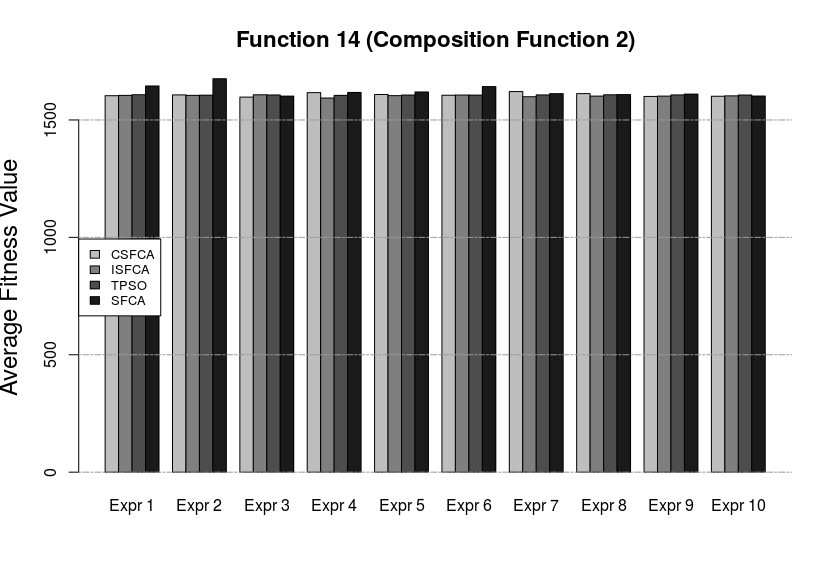
\includegraphics[scale=0.5]{func14_10}
	\centering
	\caption{Average fitness values for Function 14 with 10 dimensions}
	\label{func14_10}
\end{figure}

\begin{table}[h]
	\caption{function-14, dimension-30}
	\begin{tabular}{|c|c|c|c|c|}
		\hline
		& \textbf{SFPSO} & \textbf{CSFEP} & \textbf{SFEP} & \textbf{TPSO} \\ \hline
		\textbf{Median} & 1.675847E+03 & 1.731879E+03 & 1.820677E+03 & 1.664094E+03 \\ \hline
		\textbf{Mean} & 1.676279E+03 & 1.791878E+03 & 1.865010E+03 & 1.685711E+03 \\ \hline
		\textbf{Best} & 1.646723E+03 & 1.660532E+03 & 1.693461E+03 & 1.658174E+03 \\ \hline
		\textbf{StdDev} & 2.842502E+01 & 1.553106E+02 & 1.760265E+02 & 3.566090E+01 \\ \hline
	\end{tabular}
	\label{tbl14_30}
\end{table}
\begin{figure}[H]
	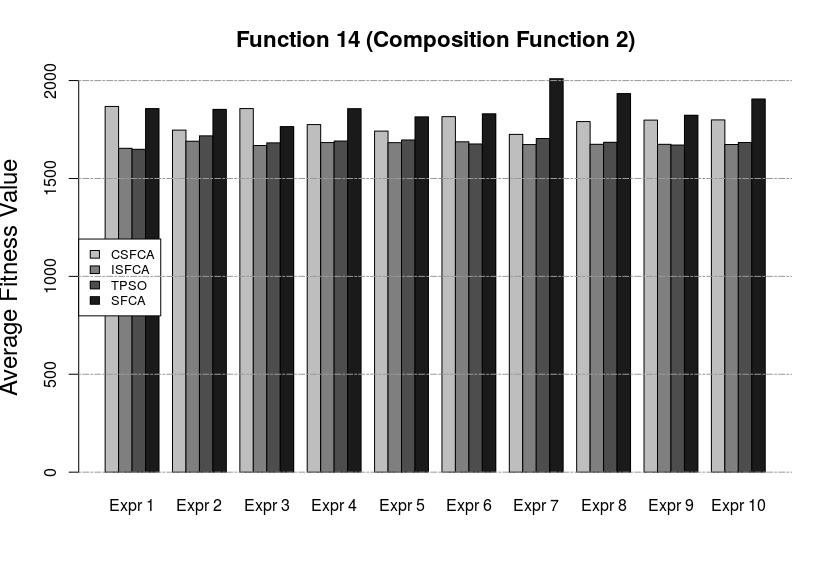
\includegraphics[scale=0.5]{func14_30}
	\centering
	\caption{Average fitness values for Function 14 with 30 dimensions}
	\label{func14_30}
\end{figure}

\section{Function 15: Composition Function 3}
For this function, ISFCA works better than CSFCA. ISFCA improves the average fitness value by 20\% and 29\% for 10- and 30-dimension cases respectively. On the other hand, CSFCA produces improvement only by 1\% and 16\% for 10- and 30-dimension cases respectively.
\begin{table}[h]
	\caption{function-15, dimension-10}
	\begin{tabular}{|c|c|c|c|c|}
		\hline
		& \textbf{SFPSO} & \textbf{CSFEP} & \textbf{SFEP} & \textbf{TPSO} \\ \hline
		\textbf{Median} & 1.560743E+03 & 1.913027E+03 & 1.949996E+03 & 1.853726E+03 \\ \hline
		\textbf{Mean} & 1.589476E+03 & 1.946018E+03 & 1.966892E+03 & 1.871080E+03 \\ \hline
		\textbf{Best} & 1.525130E+03 & 1.871689E+03 & 1.855628E+03 & 1.772940E+03 \\ \hline
		\textbf{StdDev} & 8.426385E+01 & 8.447839E+01 & 1.134500E+02 & 7.850262E+01 \\ \hline
	\end{tabular}
	\label{tbl15_10}
\end{table}

\begin{figure}[h]
	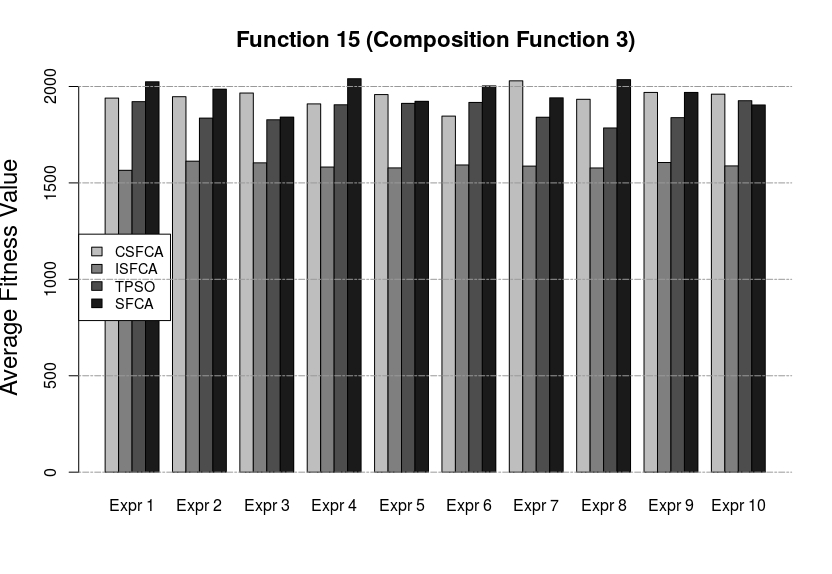
\includegraphics[scale=0.5]{func15_10}
	\centering
	\caption{Average fitness values for Function 15 with 10 dimensions}
	\label{func15_10}
\end{figure}

\begin{table}[h]
	\caption{function-15, dimension-30}
	\begin{tabular}{|c|c|c|c|c|}
		\hline
		& \textbf{SFPSO} & \textbf{CSFEP} & \textbf{SFEP} & \textbf{TPSO} \\ \hline
		\textbf{Median} & 2.565830E+03 & 2.760375E+03 & 3.096788E+03 & 2.511983E+03 \\ \hline
		\textbf{Mean} & 2.582142E+03 & 3.063021E+03 & 3.657078E+03 & 2.565208E+03 \\ \hline
		\textbf{Best} & 2.498940E+03 & 2.227419E+03 & 3.055342E+03 & 2.504910E+03 \\ \hline
		\textbf{StdDev} & 9.012990E+01 & 1.040607E+03 & 1.152769E+03 & 8.765290E+01 \\ \hline
	\end{tabular}
	\label{tbl15_30}
\end{table}
\begin{figure}[H]
	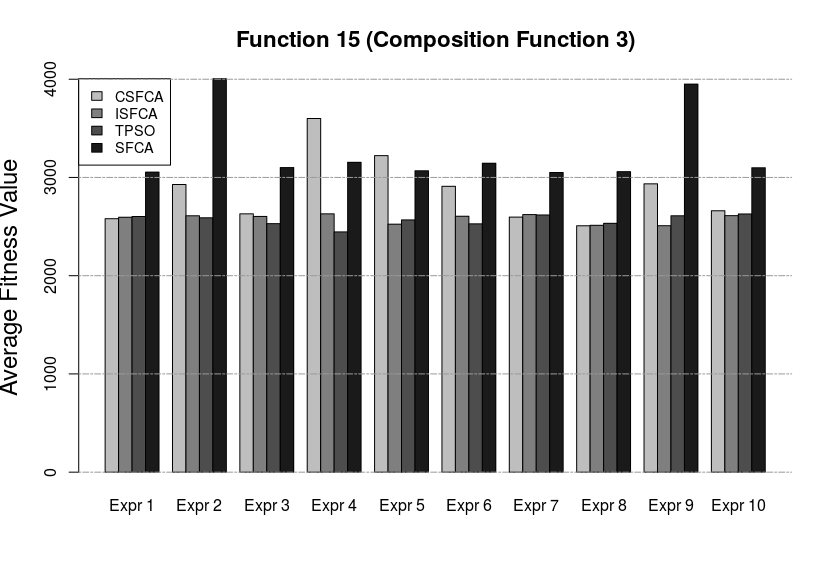
\includegraphics[scale=0.5]{func15_30}
	\centering
	\caption{Average fitness values for Function 15 with 30 dimensions}
	\label{func15_30}
\end{figure}
\section{Summary of Results}
In this chapter, we presented an extensive comparison of our proposed approaches with the standard social fabric algorithm \cite{ali2016leveraged} and Tribe-PSO \cite{chen2006tribe}. We chose these algorithms because both of them utilize multi-population and tribal strategies to improve the level of diversity in evolutionary algorithms. \newline
As we can in the tables and figures for the functions 1, 2, 8, 10, and 12, the new neighborhood restructuring strategy and the confidence-based normative ranges generated more tan 50\% improvement. It seems the proposed methods succeeded to help the individuals to avoid stagnation and local optima. \newline
For the functions 4, 7, 11, 13, 14, and 15 the new approaches improve the performance with a lower percentage between 10\% and 20\%. Although, for the remaining functions the generated improvement is trivial. We hypothesize that it occurred because of the high-level complexity of the benchmark functions we used. In the standard implementation of the IEEE-CEC2015 library, the functions are twisted and rotated to make it hard for optimization algorithms to get rid of local optima \cite{chen2014problem}. Also, as it is stated by above mentioned the No-Free Lunch Theorem,  it is not expected for an optimization algorithm to work well on all of the possible functions \cite{wolpert1997no}.
%For a Master's research this chapter represents the critical part where \textbf{you} are truly evaluated to determine whether you should be given your degree. Even more so for a PhD. Consider carefully what the University calendar states regarding the expectations for a master's thesis, paraphrased here.
%
%\begin{enumerate}
%\item {\textit{A Master�s thesis is an original lengthy essay.} The main implication here is that the essay is original, that is, it is completely newly written by you and does not contain any writings from others unless precisely quoted. Any paraphrased items must be cited.}
%\item {\textit{It must demonstrate that:}
%    \begin{itemize}
%    \item {students understand research methods;}
%    \item {students are capable to employ research methods;}
%    \item {students demonstrate command of the subject.}
%    \end{itemize}}
%\item {\textit{The work may be based on:}
%    \begin{itemize}
%    \item {original data;}
%    \item {original exercise from scholarly literature;}
%    \item {data by others.}
%    \end{itemize}}
%\item {\textit{The work must show that:}
%    \begin{itemize}
%    \item {appropriate research methods have been used;}
%    \item {appropriate methods of critical analysis supplied.}
%    \end{itemize}}
%\item {\textit{The work must contain:}
%    \begin{itemize}
%    \item {evidence of some new contribution;}
%    \item {evidence of a new perspective on existing knowledge.}
%    \end{itemize}}
%\end{enumerate}
%
%Only the last point uses the attribute \textit{new} and it refers almost entirely to giving a new perspective and analysis, even if based on data from others. This truly implies that this current chapter on evaluation and analysis of results is the most important and must be written with care. You are demonstrating here that, even if given data and methods from others, your skills of critical judgment and analysis are now at the level that you can give professional evaluations.
%
%Things are slightly different for a PhD. According to the Graduate Calendar: \\ 
%\textit{a doctoral dissertation must embody original work and constitute a significant contribution to knowledge in the candidate's field of study. It should contain evidence of broad knowledge of the relevant literature, and should demonstrate a critical understanding of the works of scholars closely related to the subject of the dissertation. Material embodied in the dissertation should, in the opinion of scholars in the field, merit publication.}
%
%\textit{The general form and style of dissertations may differ from department to department, but all dissertations shall be presented in a form which constitutes an integrated submission. The dissertation may include materials already published by the candidate, whether alone or in conjunction with others. Previously published materials must be integrated into the dissertation while at the same time distinguishing the student's own work from the work of other researchers. At the final oral examination, the doctoral candidate is responsible for the entire content of the dissertation. This includes those portions of co-authored papers which comprise part of the dissertation.}
%
%The second paragraph makes it clear that one must emphasize what is new and different from others, without arrogance, yet without being too subtle either. The first paragraph implies that for a PhD it is required that one approached an important open problem and gave a new solution altogether, making chapters 3, 4, 5 all part of the body of research being evaluated. In fact at times even the problem may be entirely new, thus including chapter 2 in the examination. This is in contrast to a Master's degree where the minimum requirement is for chapter 5 to be original.
%
%
%
%
	\startchapter{Conclusion and Future Work}
\label{concl}
\section{Conclusion}
In this thesis, two novel strategies were introduced to improve the robustness of CAs in both population and belief spaces. In the first strategy, a new neighborhood restructuring strategy is employed which aims at individuals with irregular and heterogeneous neighborhood structures. There is no centralized coordinator to control the topology of a population because the individuals are responsible for inspecting and modifying their neighborhood in a self-organized manner. Increasing the level of self-organization and autonomy is a key approach to improving robustness in a complex system.  In the second strategy, the standard implementation of normative ranges in the belief space was replaced by the confidence intervals inspired from Inferential Statistics. The new knowledge source shows a more robust search behavior to fluctuations in the input data. Now, the size of normative ranges does not change dramatically with any temporal fluctuations.\newline

\section{Future Work}
The performance of both proposed approaches is assessed through a test-suite of 15 multi-modal and hybrid functions from IEEE-CEC2015. Both methods are compared to the original version of the social fabric based CA \cite{ali2016leveraged}. The results show improvement in almost all of the functions. In some of them, the results are quite promising. Future work might be investigating the improved robustness of proposed approaches to dynamic problems or even real-world problems such as dynamic problems, data classification and social network analysis.

%My first rule for this chapter is to avoid finishing it with a section talking about future work. It may seem logical, yet it also appears to give a list of all items which remain undone! It is not the best way psychologically.

%This chapter should contain a mirror of the introduction, where a summary of the \textit{extraordinary} new results and their wonderful attributes should be stated first, followed by an executive summary of how this new solution was arrived at. Consider the practical fact that this chapter will be read quickly at the beginning of a review (thus it needs to provide a strong impact) and then again in depth at the very end, perhaps a few days after the details of the previous 3 chapters have been somehow forgotten. Reinforcement of the positive is the key strategy here, without of course blowing hot air.

%One other consideration is that some people like to join the chapter containing the analysis with the only with conclusions. This can indeed work very well in certain topics.

%Finally, the conclusions do not appear only in this chapter. This sample mini thesis lacks a feature which I regard as absolutely necessary, namely a short paragraph at the end of each chapter giving a brief summary of what was presented together with a one sentence preview as to what might expect the connection to be with the next chapter(s). You are writing a story, the \textit{story of your wonderful research work}. A story needs a line connecting all its parts and you are responsible for these linkages.

	\appendix
%	\startappendix{Additional Information}
\label{chapter:appendix}

This is a good place to put tables, lots of results, perhaps all the data compiled in the experiments. By avoiding putting all the results inside the chapters themselves, the whole thing may become much more readable and the various tables can be linked to appropriately.

The main purpose of an Appendix however should be to take care of the future readers and researchers. This implies listing all the housekeeping facts needed to continue the research. For example: where is the raw data stored? where is the software used? which version of which operating system or library or experimental equipment was used and where can it be accessed again?

Ask yourself: if you were given this thesis to read with the goal that you will be expanding the research presented here, what would you like to have as housekeeping information and what do you need? Be kind to the future graduate students and to your supervisor who will be the one stuck in the middle trying to find where all the stuff was left!



% The style of bibliography exemplified here is the "plain",
% normally used in science theses. This is shown
% by the entry {plain} below. Substitute the
% appropriate bibliography style. See also the
% PDF file "InformationOnBibliographyStyles" in this
% directory for more choices.

% The Bibliography file is a BibTex file named
% UVicThesis.bib and called below

	\TOCadd{Bibliography}
	%\bibliographystyle{plain}%{macros/aaai}
	\bibliographystyle{plainnat}
	\bibliography{UvicThesis}

\end{document}
